\chapter{Experiments \& Results} 
\label{chapter-experiments} 

This chapter experimentally verifies the main ideas discussed in the previous chapters \ref{chapter-energy-estimation} and \ref{chapter-emma}. In chapter \ref{chapter-energy-estimation}, the derivation of the potential energy from an autoencoder was shown, with the potential energy being proportional to the log-likelihood. We claimed that this metric could be used to distinguish normal samples from failing ones. On the other hand, chapter \ref{chapter-emma} described the design of EMMA, which is constructed to change the allocation of its attention in the face of varying levels of perturbations, and thus improving the robustness of the MMN. 

%----------------------------------------------------------------------------------------
%	SECTION 
%----------------------------------------------------------------------------------------

\section{Pulsar Stars}
For the following experiments, our models will be trained on the HTRU2 dataset\footnote{The dataset can be found \href{https://archive.ics.uci.edu/ml/datasets/HTRU2}{here}, and was collected by \citep{HTRU}}, containing features describing radio emissions measured on Earth. The positive class corresponds to radio emissions of pulsars, which are a rare type of Neutron star that produce radio emissions detectable here on Earth, whereas the negative class corresponds to the other radio emissions. Pulsars are of considerable scientific interest as probes of gravitational theories and time-keeping systems in spacecraft. A short summary of the seminal work of \citep{lyon} on this subject can be found in Appendix \ref{chapter-dataset}. 

The models will learn to distinguish pulsars from other radio emissions. The dataset consists of two modes:
\begin{itemize}
\item \textit{integrated profile} (IP): each pulsar produces a unique pattern of pulse emissions. The integrated profile is an average of these patterns over many thousands of rotations (further details in Appendix \ref{chapter-dataset}). The mode contains four features, namely the mean, standard deviation, excess kurtosis\footnote{Kurtosis refers to the size of the tails of a distribution. Excess kurtosis is a measure of how prone the distribution is to extreme outcomes.} and skewness of the integrated profile.
\item \textit{dispersion measure} (DM): the amount of dispersive smearing\footnote{See Appendix \ref{chapter-dataset}.} a signal receives is proportional to a quantity called the dispersion measure, which is the integrated column density of free electrons between an observer and a pulsar (further details in Appendix \ref{chapter-dataset}). Similarly, the mode contains four features, namely the mean, standard deviation, excess kurtosis and skewness of the dispersion measure.
\end{itemize}

An additional difficulty of this dataset is that it is skewed, there are approximately ten time less positive samples than negative ones ($17.898$ total samples, $1.639$ positive samples, $16.259$ negative samples). This issue was handled by imposing a penalty in the loss function to fight the class imbalance.

In the experiments, the dataset will be split into training, validation and test sets (see Table \ref{tab:split}). The validation set is used for tuning purposes, and to implement an Early Stopping\footnote{Early stopping \citep{early-stopping} is a form of regularization to avoid overfitting, where the error on the validation set is used in determining when overfitting has begun i.e., when the validation error starts increasing.} algorithm. Usually, the model is then retrained for a few iterations on both the combined training and validation set. In the case at hand, for the sake of simplicity, the model is not retrained on the combined sets. Prior to the training, the data is standardized for the purpose of having the same noise-to-signal ratio corruption effect on all features, since all their variances are equal to one. To avoid information leakage, the statistics (i.e., mean and variance) for the standardization are computed from the training set instead of the entire dataset, and applied to the three data subsets. 
\begin{table}
\centering
\begin{tabular}{ r|cc|c } 
  & positive & negative & total \\ 
 \hline \hline
 train & 1.098 & 10.894 & 11.992 \\
 validation & 270 & 2.683 & 2.953 \\  
 test & 271 & 2.682 & 2.953 \\ 
 \hline
 total & 1.639 & 16.259 & 17.898 \\ 
 \hline
\end{tabular}
 \caption{Number of samples per split/class of the pulsar dataset.}
\label{tab:split}
\end{table}

%----------------------------------------------------------------------------------------
%	SECTION 
%----------------------------------------------------------------------------------------

\section{Experiment I}\label{sec:expII}
To verify whether the potential energy is a good measure of failure intensity, one autoencoder per mode was trained on the training set. Next, these autoencoders were evaluated on the test set, which partially contained noisy or out-of-distribution samples. The objective is to assess whether a clear difference in the potential energy values is recorded for the failing modes compared to that of regular ones. Notably, missing values are implicitly solved by replacing them by zeros\footnote{$\beta\cdot 0 = 0,\,\forall \beta \in \mathbb{R}$}. With this in mind, we did not evaluate missing modes. 

\subsection*{Noisy values}
To simulate noise, Gaussian white noise $\mathcal{N} \sim (0, \sigma_{\mbox{corruption}}^2)$ is added to the test set. Then, the mean and variance of potential energies obtained for all samples are computed. This process is then repeated for different noise intensities. The results for each mode are shown in Figure \ref{fig:pot-noisy-signal}, which confirms that the potential energy can capture the noise in test data, relative to training samples.
\begin{figure}[!h]
\centering
\begin{subfigure}{.5\textwidth}
  \centering
  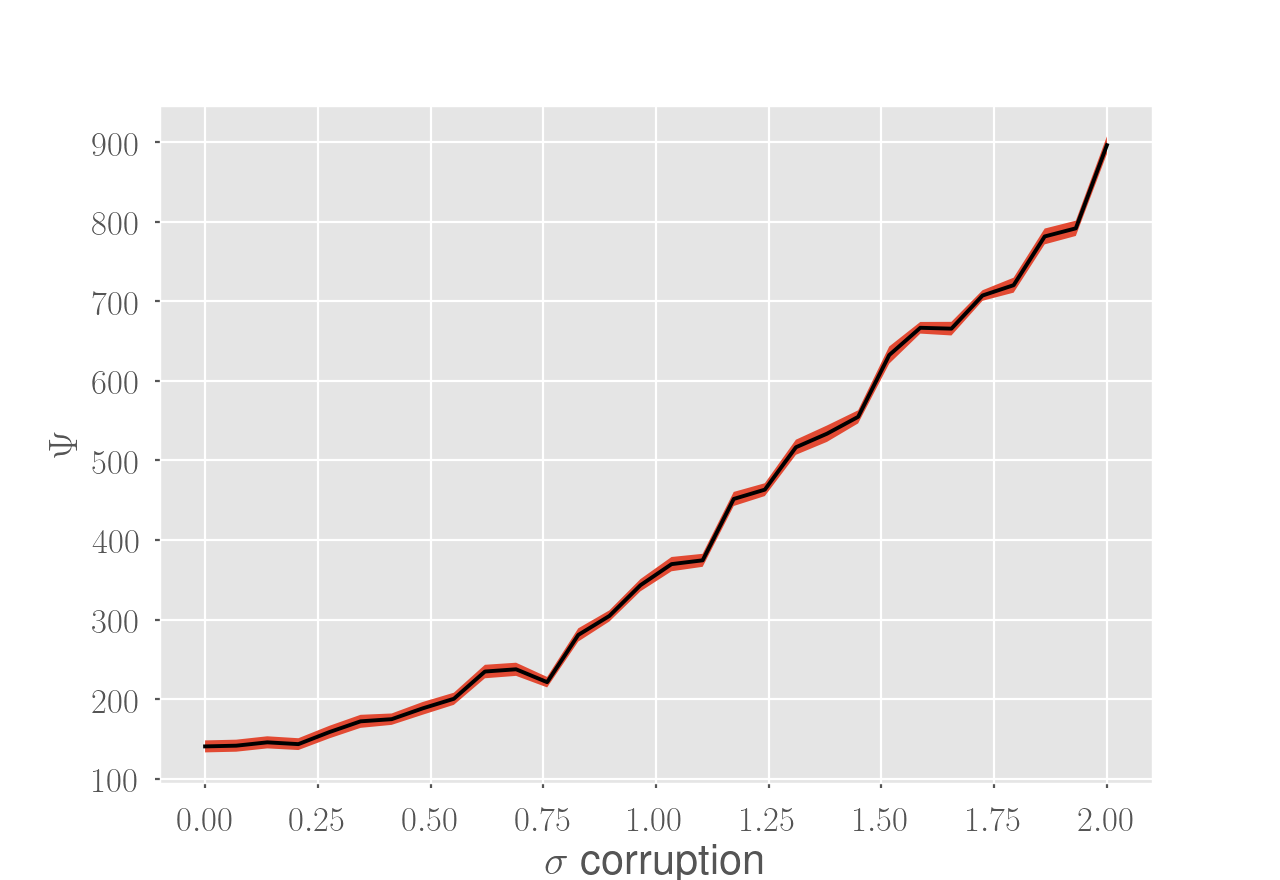
\includegraphics[width=\linewidth]{figures/noisy-signal-ip}
  \caption{IP mode}
\end{subfigure}%
\begin{subfigure}{.5\textwidth}
  \centering
  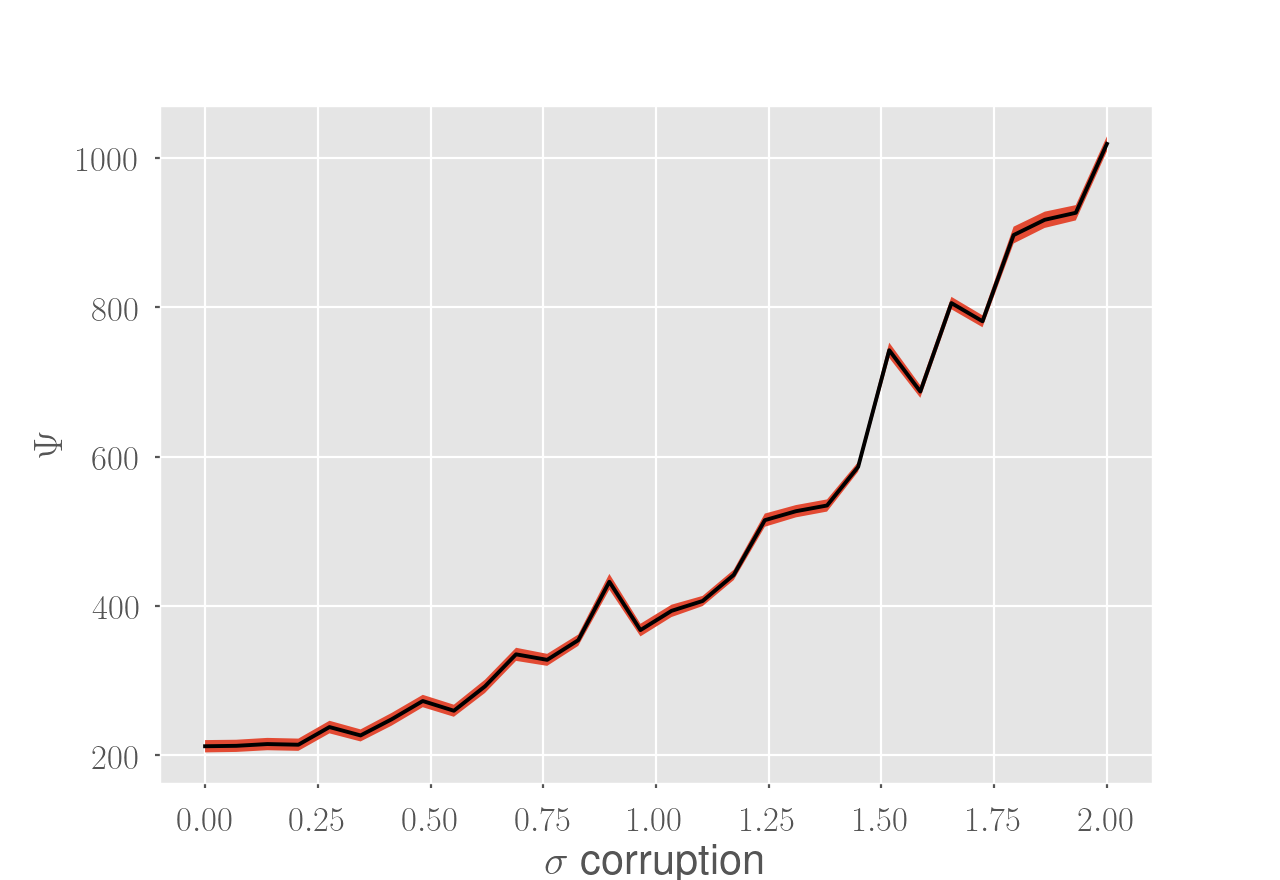
\includegraphics[width=\linewidth]{figures/noisy-signal-dm-snr}
  \caption{DM mode}
\end{subfigure}
\caption[Potential energy measured on noisy test samples]{Potential energy measured on noisy test samples (the mean corresponds to the black line, whereas the interval of two times the standard deviation error is displayed in red).}
\label{fig:pot-noisy-signal}
\end{figure}

\subsection*{Out-of-distribution samples}
Since only two classes are considered in this experiment, the conventional procedure whereby autoencoders are trained on all samples is altered, such that the training set only includes positive samples. In this case, negative samples can therefore be considered as being out-of-distribution. As can be seen from Figure \ref{fig:pot-oof-signal}, the potential energies computed on the test set (containing both positive and negative samples) allow to distinguish fairly well between positive and negative samples. Indeed, in most cases, the potential energies of likely data (positive samples) are noticeably lower than that of unlikely data (negative samples). This pattern is consistent with energy-based models described in Section \ref{sec:ebm}.
\begin{figure}[!h]
\centering
\begin{subfigure}{.5\textwidth}
  \centering
  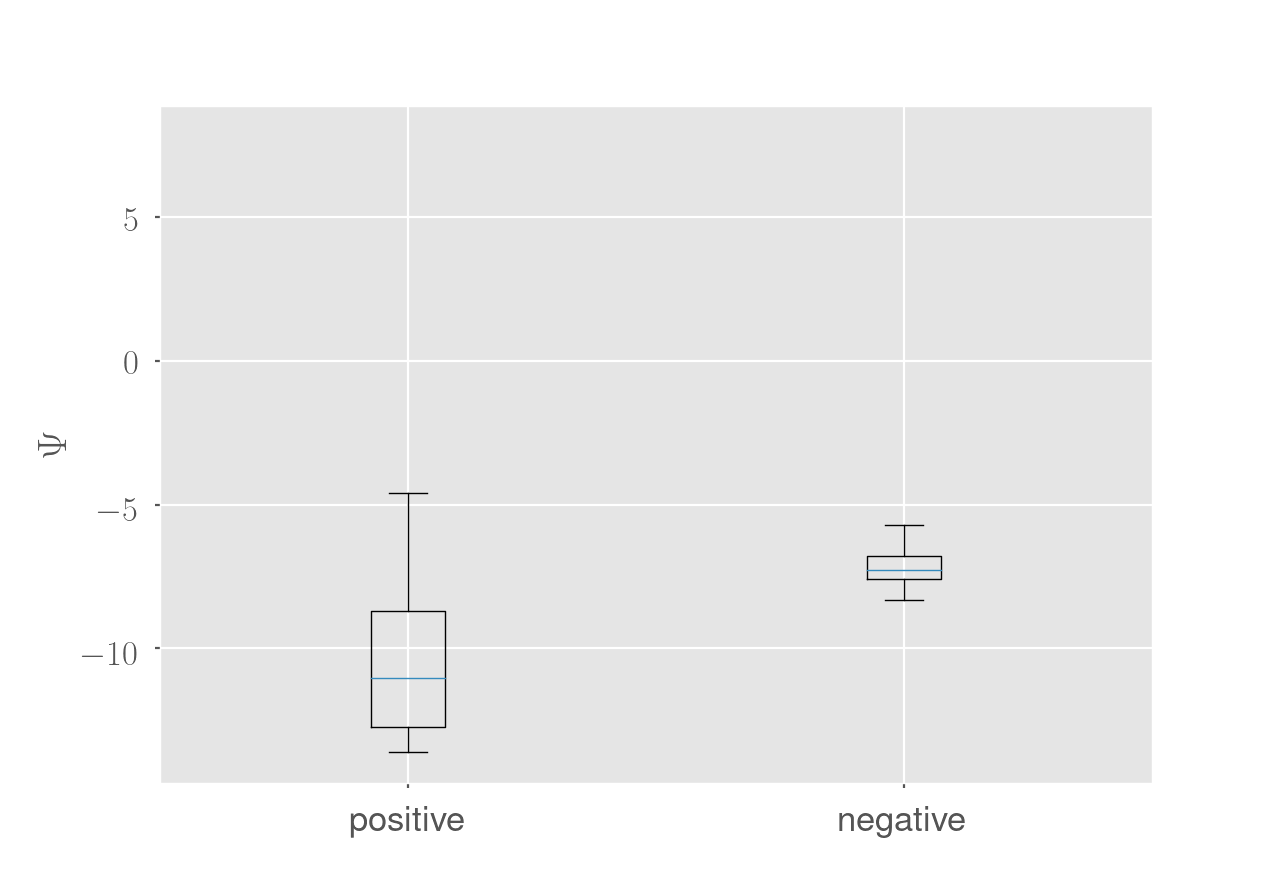
\includegraphics[width=\linewidth]{figures/signal-vs-background-ip}
   \caption{IP mode}
\end{subfigure}%
\begin{subfigure}{.5\textwidth}
  \centering
  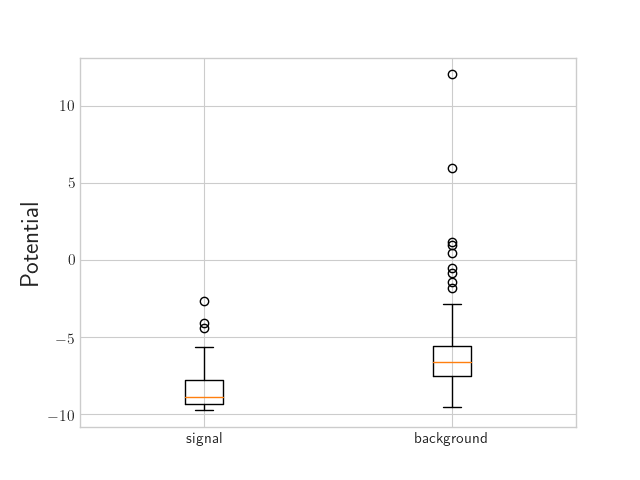
\includegraphics[width=\linewidth]{figures/signal-vs-background-dm-snr}
   \caption{DM mode}
\end{subfigure}
\caption[Potential energy measured on out-of-distribution samples]{Potential energy measured on positive and negative samples, derived from autoencoders only trained on positive samples.}
\label{fig:pot-oof-signal}
\end{figure}


%----------------------------------------------------------------------------------------
%	SECTION 
%----------------------------------------------------------------------------------------

\newpage\section{Experiment II}\label{sec:expIII} 

\subsection{Description}

The motivation of this experiment is to show the effect of the attention module on the inputs, and its effectiveness in improving the robustness of the MMN. To this end, failing modes are simulated by adding white noise. The predictions of the model fitted with EMMA are compared with the predictions of models having the same architecture but without EMMA. The reason only noisy failing types are tested is two-fold. First, conventional models are generally not able to spontaneously learn to detect out-of-distribution samples. Secondly, it is straightforward to control the intensity of the failing mode by changing the noise-to-signal ratio. 

To asses the extent to which fitting EMMA to a standard MMN can improve its predictive performance and robustness, the performance of the coupled models is compared with that of i) a stand-alone MMN ii) a stand-alone MMN trained via a standard data augmentation technique, which consists in adding noisy samples to the training set in the hope that the MMN learns to suppress the noise by itself. In summary, six types of models are evaluated:
\begin{itemize}
\item \texttt{IP-only} is a small MMN trained on samples containing only data from the IP-mode.
\item \texttt{DM-only} is a small MMN trained on samples containing only data from the DM-mode.
\item \texttt{base-model} is the MMN optimized on the training set (stage 1). Thus, without added noise neither using EMMA.
\item \texttt{model-without} is the model initialized with the weights of the \texttt{base-model}, and finetuned on a mix of corrupted and uncorrupted samples of the training set (data augmentation technique).
\item \texttt{alternative} is the \texttt{base-model} coupled with an alternative attention module \citep{audiovisual-attention}, discussed in the literature review, finetuned on a mix of corrupted and uncorrupted samples.
\item \texttt{model-with} is the combined \texttt{base-model} with the attention module EMMA. This model is trained end-to-end on a mix of corrupted and uncorrupted data (stage 2). 
\end{itemize}
The corruption process is applied as follows to each data subset separately: 50\% of the samples stay uncorrupted, 25\% of the samples are corrupted only on the IP mode and for the remaining samples only the DM mode is corrupted. In particular, the samples are corrupted by adding Gaussian white noise with a $\sigma_{\text{corruption}} = 0.5$.

The chosen loss function is the binary cross-entropy with an imbalance penalty\footnote{The imbalance penalty weights the loss of each sample with respect to the proportion of its corresponding class in the dataset}. Moreover, the three types of models are trained for 30 epochs with Early Stopping, implemented in the following way: at each epoch the state of the current model is saved as the new optimal one if the validation  error is lower than the previous minimum. Furthermore, the optimal classification threshold is determined on the validation set using the receiver operating characteristic (ROC) curve. Lastly, the F1-score is used as the criterion to evaluate the performance on the test set. 

\subsection{Results}
Table \ref{tab:results} shows the F1-scores of the three types of models on both corrupted and uncorrupted samples of the test set. For the \texttt{model-with}, 125 combinations of hyperparameters were trained, from which the fifteen best ones were extracted and shown in Table \ref{tab:results}. As expected, the \texttt{base-model} performs badly on samples with a noisy mode, since it was only trained on uncorrupted data. Furthermore, the results of \texttt{model-without} indicate that using data augmentation indeed improves the performance on noisy data, whereas the performance on uncorrupted samples slightly decreases. On the other hand, models equipped with the attention module (\texttt{model-with}) consistently outperform \texttt{model-without} and \texttt{base-model} on noisy data by a significant margin. Somewhat surprisingly, using the attention module appears to slightly improve the F1-score on uncorrupted data as well compared to the \texttt{base-model}. A possible explanation could be that EMMA is able to capture a small spectrum of quality about the training data, which would then be used by the MMN to improve the predictions. Nevertheless, further investigation is required to validate this hypothesis. Lastly, it is worth noticing that the models seems to be more robust against one failing mode (DM) then the other (IP). Since the noise-to-signal ratios are uniform across modes, it could be hypothesized that the latter mode is more informative. This hypothesis is verified by the obtained performance of the models \texttt{IP-only} and \texttt{DM-only}.
\begin{table*}\centering
\ra{1.3}
\begin{tabular}{@{}rrrrcrrr@{}}\toprule
& \multicolumn{3}{c}{Hyperparameters} & \phantom{abc}& \multicolumn{3}{c}{F1-score}\\
\cmidrule{2-4} \cmidrule{6-8}
& \multicolumn{1}{c}{$\rho$} & \multicolumn{1}{c}{$\lambda_c$} & \multicolumn{1}{c}{$\lambda_e$} && \multicolumn{1}{r}{uncorrupted} & \multicolumn{1}{r}{IP noisy} & \multicolumn{1}{r}{DM noisy}\\ \midrule\midrule
IP-only & & & && 0.8235 & 0.5926 & \\
DM-only & & & && 0.6612 &  & 0.3920\\\midrule
base & & & && 0.8830 & 0.6441 & 0.6569\\
without & & & && 0.8671& 0.7097& 0.7683\\
alternative & & & && 0.7726 & 0.6129 & 0.6882\\\midrule
with & $10^{-4}$ & $10^{-3}$ & $10^{-2}$ && $\mathbf{0.8881}$& $\mathbf{0.7333}$& $\mathbf{0.8077}$\\
with & $10^{-4}$ & $0$ & $10^{-2}$ && $\mathbf{0.8849}$& $\mathbf{0.7285}$& $\mathbf{0.8183}$\\
with & $10^{-4}$ & $10^{-4}$ & $10^{-2}$ && $\mathbf{0.8945}$& $\mathbf{0.7333}$& $\mathbf{0.8182}$\\
with & $10^{-3}$ & $10^{-3}$ & $0$ && 0.8809& $\mathbf{0.7347}$& $\mathbf{0.8186}$\\
with & $10^{-4}$ & $10^{-2}$ & $10^{-3}$ && 0.8736& $\mathbf{0.7383}$& $\mathbf{0.7848}$\\
with & $10^{-1}$ & $10^{-2}$ & $0$ && 0.8826& $\mathbf{0.7467}$& $\mathbf{0.7925}$\\
with & $10^{-4}$ & $10^{-3}$ & $0$ && 0.8786& $\mathbf{0.7190}$& $\mathbf{0.7826}$\\
with & $10^{-3}$ & $10^{-1}$ & $10^{-2}$ && 0.8800& $\mathbf{0.7432}$& $\mathbf{0.8344}$\\
with & $10^{-4}$ & $0$ & $10^{-4}$ && 0.8723& 0.7051& $\mathbf{0.7853}$\\
with & $10^{-4}$ & $10^{-4}$ & $10^{-3}$ && 0.8794& 0.7053& $\mathbf{0.7853}$\\
\bottomrule
\end{tabular}
\caption{F1-scores of the top-10 trained \texttt{model-with} (the models are ranked by their weighted average F1-score) along with the other types of models.}
\label{tab:results}
\end{table*}

\subsection*{Attention allocation and shifts}
A key feature of EMMA is to allocate its attention toward the most important modes. The validity of this claim can be ascertained by monitoring the change in allocation under various circumstances. As a reminder, the importance and attention scores introduced in Section \ref{sec:general-framework} can be leveraged allowing us to evaluate the attention change. These scores are reported in Figure \ref{fig:exp-att-shift-1} for two levels of noise, and clear changes in allocation can be observed as a result of the application of noise onto the different modes. Interestingly, it can be seen in Figure \ref{fig:exp-att-shift-1-a} that for low levels of noise applied to the IP mode, it still receives more attention than the DM mode. This is consistent with the aforementioned observation that the IP-mode seems to be more informative. In contrast, if the noise level on this mode is sufficiently increased (Figure \ref{fig:exp-att-shift-1-c}), an attention shift occurs and the other mode becomes more important. A more complete view of the attention scores for varying levels of noise applied to different modes is given in Figure \ref{fig:mesh}.
\begin{figure}[!h]
\centering
\begin{subfigure}{.5\textwidth}
  \centering
  \includegraphics[width=\linewidth]{figures/noise-0-5/alpha-distrib-0}
  \caption{importance, noise $\sigma=0.5$} 
  \label{fig:exp-att-shift-1-a}
\end{subfigure}%
\begin{subfigure}{.5\textwidth}
  \centering
  \includegraphics[width=\linewidth]{figures/noise-0-5/beta-distrib-0}
  \caption{attention, noise $\sigma=0.5$} 
  \label{fig:exp-att-shift-1-b}
\end{subfigure}
\begin{subfigure}{.5\textwidth}
  \centering
  \includegraphics[width=\linewidth]{figures/noise-2/alpha-distrib-0}
  \caption{importance, noise $\sigma=2$}
  \label{fig:exp-att-shift-1-c} 
\end{subfigure}%
\begin{subfigure}{.5\textwidth}
  \centering
  \includegraphics[width=\linewidth]{figures/noise-2/beta-distrib-0}
  \caption{attention, noise $\sigma=2$} 
  \label{fig:exp-att-shift-1-d}
\end{subfigure}
\caption[Importance and attention scores for the $1^{\text{st}}$ ranked model]{Importance and attention scores for the $1^{\text{st}}$ ranked \texttt{model-with} ($\rho=10^{-4},\,\lambda_e=10^{-3},\,\lambda_c=10^{-2}$), on two different levels of noises ($\sigma=0.5$ and $\sigma=2$).}
\label{fig:exp-att-shift-1}
\end{figure}
\begin{figure}[!h]
\centering
\begin{subfigure}{\textwidth}
  \centering
  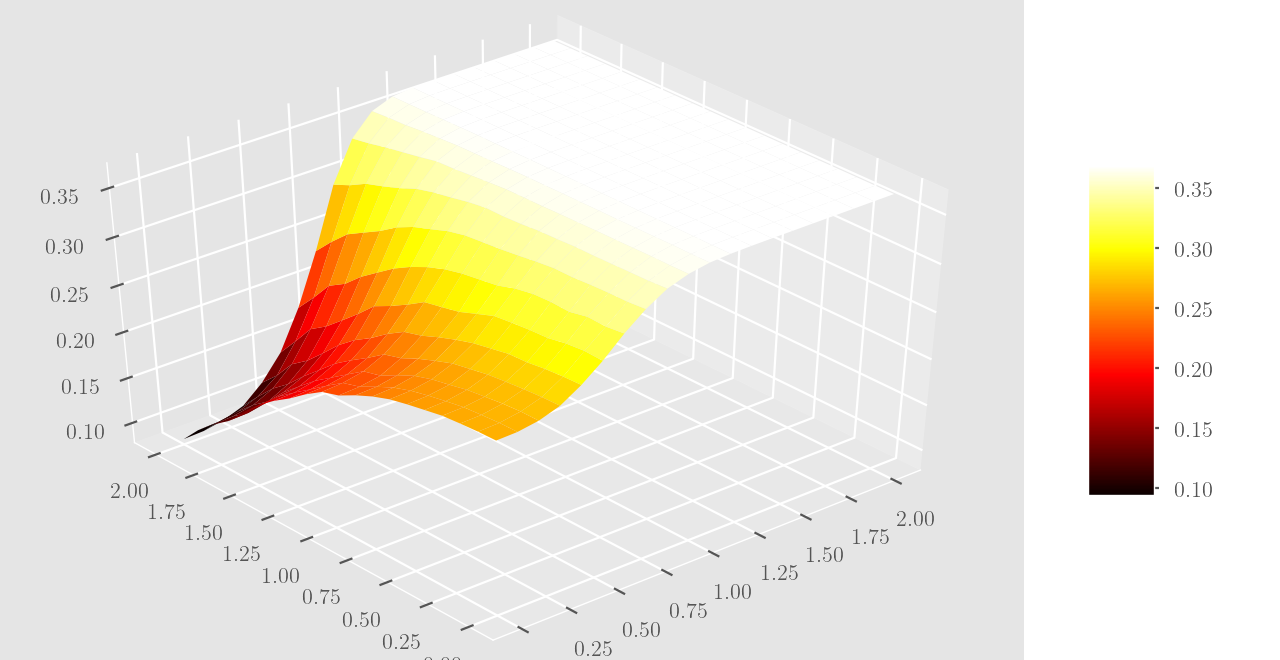
\includegraphics[scale=0.25]{figures/Figure_1} 
  \caption{$\beta$-ip}
\end{subfigure}\\
\begin{subfigure}{\textwidth}
  \centering
  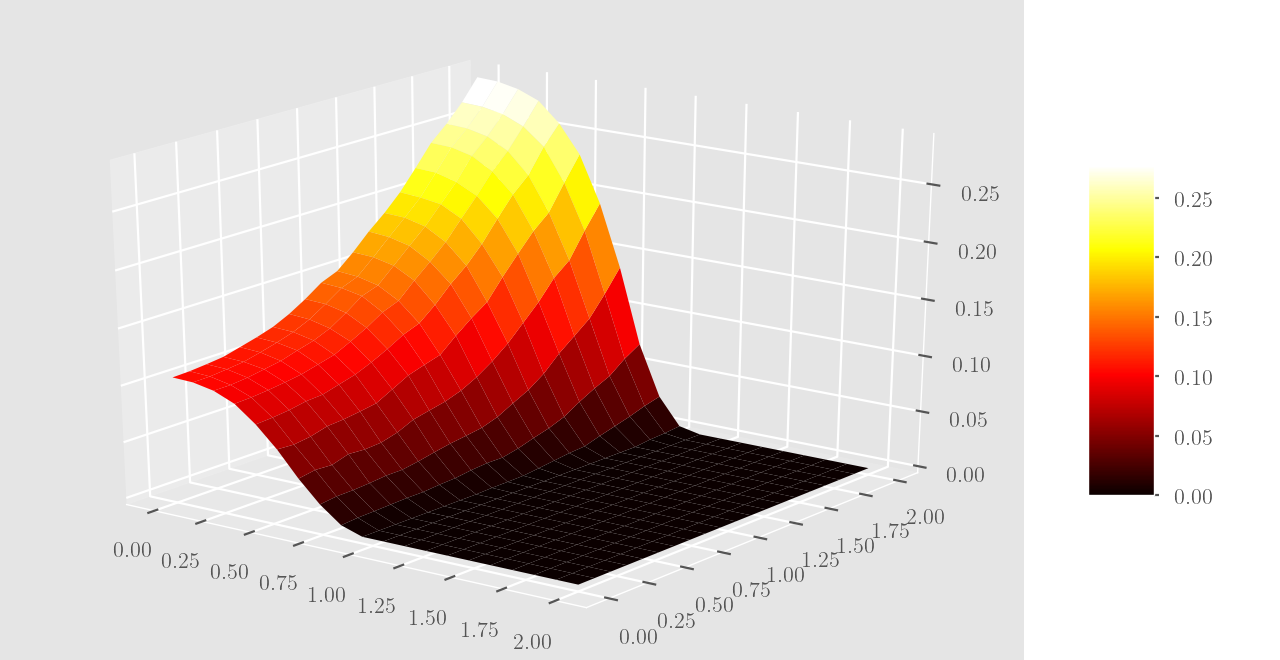
\includegraphics[scale=0.25]{figures/Figure_2} 
  \caption{$\beta$-dm}
\end{subfigure}
\caption[3D visualization of attention scores on varying levels of noises]{3D visualization of attention scores on varying levels of noises between the modes of the same model as Figure \ref{fig:exp-att-shift-1}. The axis in the horizontal plane represent the variance of noise on each modes, whereas the vertical axis corresponds to the attention score.}
\label{fig:mesh}
\end{figure}

To gain a better understanding of the attention allocation, it is worth further investigating the role of the coldness hyperparameter ($\rho$, see Section \ref{sec:step3}). A simple way of doing so consists in comparing the importance scores of models trained with significantly different temperatures as displayed in Figure \ref{fig:exp-att-shift-2-a} and \ref{fig:exp-att-shift-2-c}. As expected, the values of the importance scores are more uniformly distributed for the one with a high temperature (Figure \ref{fig:exp-att-shift-2-a}), permitting the module to stay more stable for higher levels of noise (Figure \ref{fig:exp-att-shift-2-b}). Indeed, it was proved that an increase of the overall perturbation level makes the module more selective (see the \textit{energy threshold} explained in Section \ref{sec:capacity}) On the contrary, the model trained with a lower temperature has more pronounced attention shifts (Figure \ref{fig:exp-att-shift-2-c}). As a result, the corrupted mode will be masked very rapidly, and discarded altogether for high levels of noise (seen in Figure \ref{fig:exp-att-shift-2-d}). Another view of the same example is given in Figure \ref{fig:exp-att-shift-3}, where instead the attention scores are visualised on a continuum of noise intensities. It can be seen that the model with the high temperature (Figure \ref{fig:exp-att-shift-3-a} and \ref{fig:exp-att-shift-3-b}) is able to learn a richer attention profile than the one with the low temperature (Figure \ref{fig:exp-att-shift-3-c} and \ref{fig:exp-att-shift-3-d}). Indeed, the crossing-point in Figure \ref{fig:exp-att-shift-3-a} corresponding to the attention shift, may be interpreted as the trade-off between the relevance and failure intensity. In contrast, the other module having a low temperature is naturally more biased towards the uncorrupted mode, limiting the training process and making it more difficult to learn the interactions between the modes. These results also visually confirm the utility of multiplying the modes by attention scores instead of importance scores. Indeed, in Figure \ref{fig:exp-att-shift-3-c} and \ref{fig:exp-att-shift-3-d} the module learns to allocate a high attention to both modes for low levels of noise and is still able to mask out the corrupted mode if the noise-to-signal ratio increases. This behaviour can not be modelled if we multiply the modes by the attention scores, since they sum up to one.
\begin{figure}[!h]
\centering
\begin{subfigure}{.5\textwidth}
  \centering
  \includegraphics[width=\linewidth]{figures/noise-0-5/alpha-distrib-4}
  \caption{importance, $\rho=10^{-4}$, noise $\sigma=0.5$} 
  \label{fig:exp-att-shift-2-a}
\end{subfigure}%
\begin{subfigure}{.5\textwidth}
  \centering
  \includegraphics[width=\linewidth]{figures/noise-2/alpha-distrib-4}
  \caption{importance, $\rho=10^{-4}$, noise $\sigma=2$} 
  \label{fig:exp-att-shift-2-b}
\end{subfigure}
\begin{subfigure}{.5\textwidth}
  \centering
  \includegraphics[width=\linewidth]{figures/noise-0-5/alpha-distrib-5}
  \caption{importance, $\rho=10^{-1}$, noise $\sigma=0.5$} 
  \label{fig:exp-att-shift-2-c}
\end{subfigure}%
\begin{subfigure}{.5\textwidth}
  \centering
  \includegraphics[width=\linewidth]{figures/noise-2/alpha-distrib-5}
  \caption{importance, $\rho=10^{-1}$, noise $\sigma=2$} 
  \label{fig:exp-att-shift-2-d}
\end{subfigure}
\caption[Importance scores comparison of models with different temperatures]{Importance scores comparison of models with different temperatures: \texttt{model-with} ($\rho=10^{-4},\,\lambda_e=10^{-2},\,\lambda_c=10^{-3}$) and \texttt{model-with} ($\rho=10^{-1},\,\lambda_e=10^{-2},\,\lambda_c=10^{-3}$).}
\label{fig:exp-att-shift-2}
\end{figure}

\begin{figure}[!h]
\centering
\begin{subfigure}{.5\textwidth}
  \centering
  \includegraphics[width=\linewidth]{figures/noise-generalisation-ip-noisy-beta-4}
  \caption{attention, $\rho=10^{-4}$, noise on IP} 
  \label{fig:exp-att-shift-3-a}
\end{subfigure}%
\begin{subfigure}{.5\textwidth}
  \centering
  \includegraphics[width=\linewidth]{figures/noise-generalisation-dm-noisy-beta-4}
  \caption{attention, $\rho=10^{-4}$, noise on DM} 
  \label{fig:exp-att-shift-3-b}
\end{subfigure}
\begin{subfigure}{.5\textwidth}
  \centering
  \includegraphics[width=\linewidth]{figures/noise-generalisation-ip-noisy-beta-5}
  \caption{attention, $\rho=10^{-1}$, noise on IP} 
  \label{fig:exp-att-shift-3-c}
\end{subfigure}%
\begin{subfigure}{.5\textwidth}
  \centering
  \includegraphics[width=\linewidth]{figures/noise-generalisation-dm-noisy-beta-5}
  \caption{attention, $\rho=10^{-1}$, noise on DM} 
  \label{fig:exp-att-shift-3-d}
\end{subfigure}
\caption[Attention scores comparison of models with different temperatures]{Attention scores comparison of models with different temperatures: \texttt{model-with} ($\rho=10^{-4},\,\lambda_e=10^{-2},\,\lambda_c=10^{-3}$) and \texttt{model-with} ($\rho=10^{-1},\,\lambda_e=10^{-2},\,\lambda_c=10^{-3}$). The learned capacity\footnote{Computed with Equation (\ref{eq:capacity}).} for these models are respectively 0.49 and 0.63.}
\label{fig:exp-att-shift-3}
\end{figure}

\clearpage\subsection*{Total Energy}\label{sec:total-energy}
As mentioned in Chapter \ref{chapter-emma}, one of the key advantages of the attention module is to facilitate/promote results interpretability. In particular, a quantity named the total energy, which can be computed as the sum of all modal energies of a given sample, provides readily interpretable clues pertaining to the workings of the model. By construction, the total energy captures the overall amount of perturbation in a given sample, and can thus serve as a good proxy for quantifying the uncertainty on the predictions at test time.

In order to evaluate the veracity of this claim, the following experiment is carried out. Firstly, both modes are corrupted in the test set. Then, the total energy and F1-score are computed for each sample, and averaged over the entire test set. This process is then repeated for increasing noise intensities. The results are shown in Figure \ref{fig:exp-att-shift-5}. A significant correlation can indeed be observed between the total energy and the F1-score. Remarkably, this pattern is observed for all the modules, independently of the chosen set of hyperparameters. Hence, the total energy could indeed be used as a proxy for uncertainty on the predictions. 
\begin{figure}[H]
\centering
\begin{subfigure}{.5\textwidth}
  \centering
  \includegraphics[width=\linewidth]{figures/noise-vs-system-energy}
\end{subfigure}%
\begin{subfigure}{.5\textwidth}
  \centering
  \includegraphics[width=\linewidth]{figures/noise-vs-system-f1}
\end{subfigure}
\caption[Total energy]{Total energy for \texttt{model-with} ($\rho=10^{-4},\,\lambda_e=10^{-3},\,\lambda_c=10^{-2}$).}
\label{fig:exp-att-shift-5}
\end{figure}

\subsection*{Robustness Generalisation}\label{sec:generalization}
As discussed in Chapter \ref{chapter-literature-review}, the robustness of a model is often evaluated under the same conditions as the training. This approach appears somewhat questionable. Indeed, the conditions under which the model will be deployed cannot, in most cases,  be specified exactly in advance. In particular, the nature and occurrence of failing modes may be unknown \textit{a priori}. As a result, it appears very likely that such an evaluation method provides an overly optimistic assessment of model robustness.

In this study, in order to carry out a more realistic robustness assessment of the combined model (\texttt{model-with}), the quality of the predictions is evaluated on test sets with varying levels of noises. In particular, \textit{only one mode} of the test set is corrupted with a specific intensity of noise on which the model is evaluated. This process is then repeated for increasing noise intensity. The results of the robustness analysis of the $1^\text{st}$ ranked model are shown In Figure \ref{fig:exp-att-shift-6}. When the noise is applied on the DM-mode (Figure \ref{fig:exp-att-shift-6-b}), he performance of the \texttt{model-with} remain more stable than that of the other models. The masking of the noise by the attention module is verified in Figure \ref{fig:exp-att-shift-6-d}. \textit{TODO: rewrite with new findings.}


\begin{figure}[!h]
\centering
\begin{subfigure}{.5\textwidth}
  \centering
  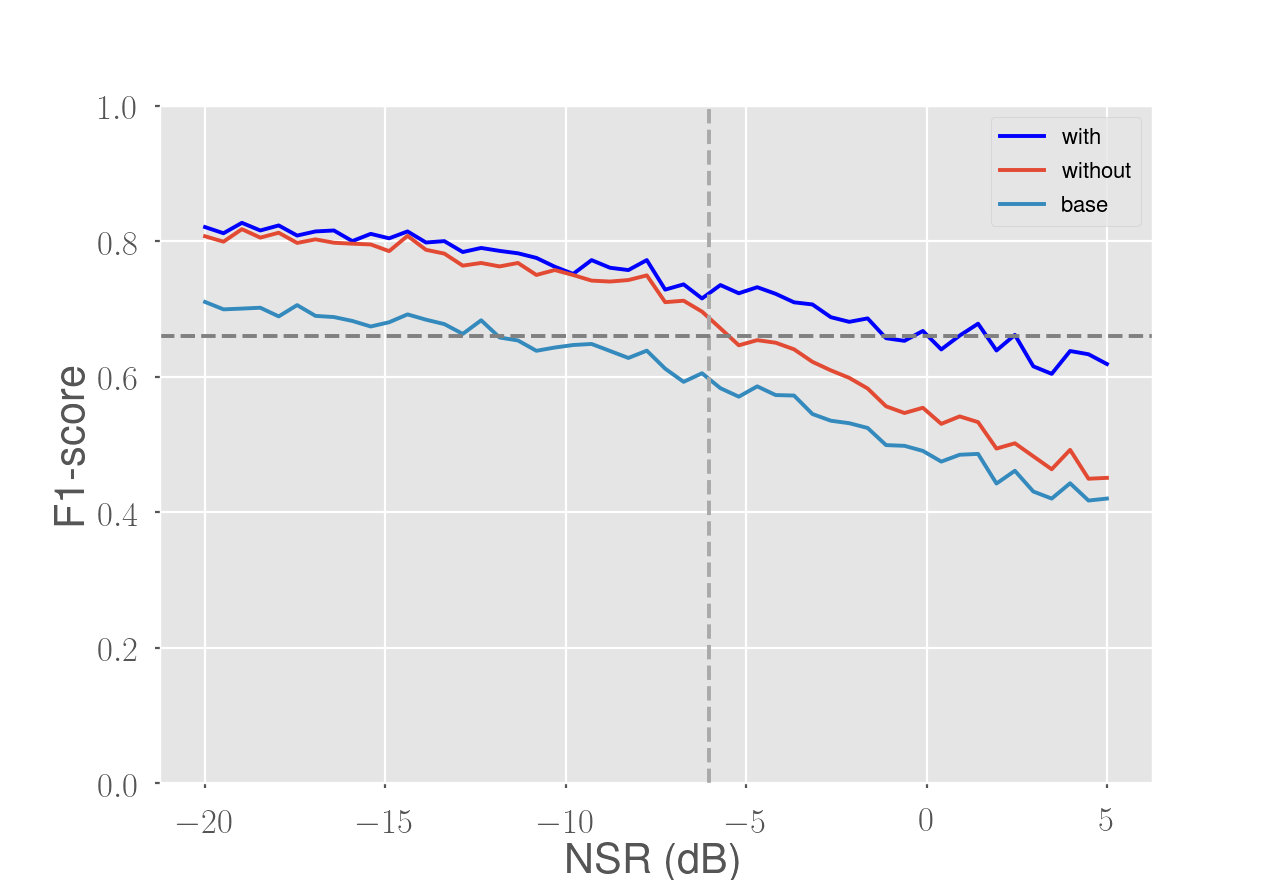
\includegraphics[width=\linewidth]{figures/new/noise-generalisation-ip-noisy}
  \caption{F1-score, noisy IP-mode}
  \label{fig:exp-att-shift-6-a}
\end{subfigure}%
\begin{subfigure}{.5\textwidth}
  \centering
  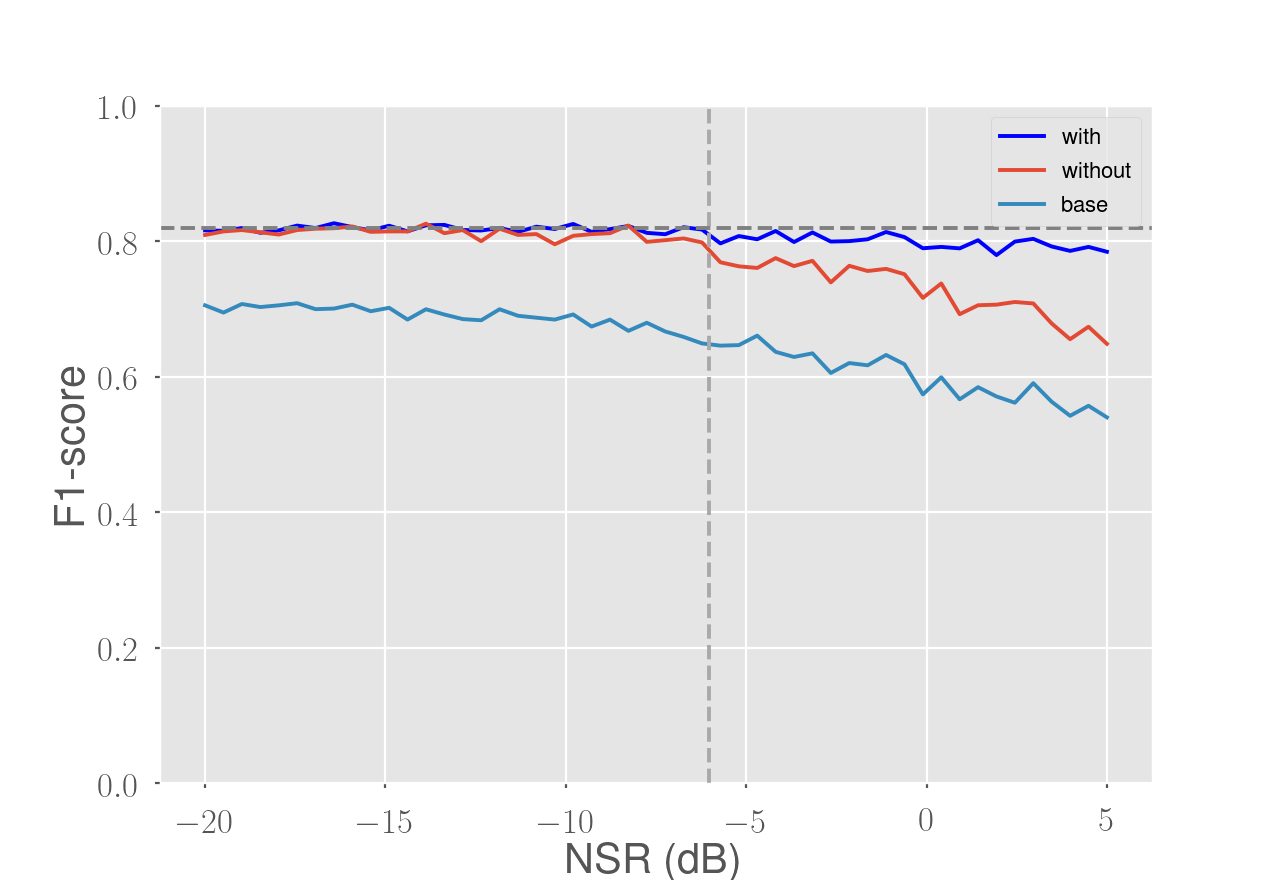
\includegraphics[width=\linewidth]{figures/new/noise-generalisation-dm-noisy}
  \caption{F1-score, noisy DM-mode}
 \label{fig:exp-att-shift-6-b} 
\end{subfigure}
\begin{subfigure}{.5\textwidth}
  \centering
  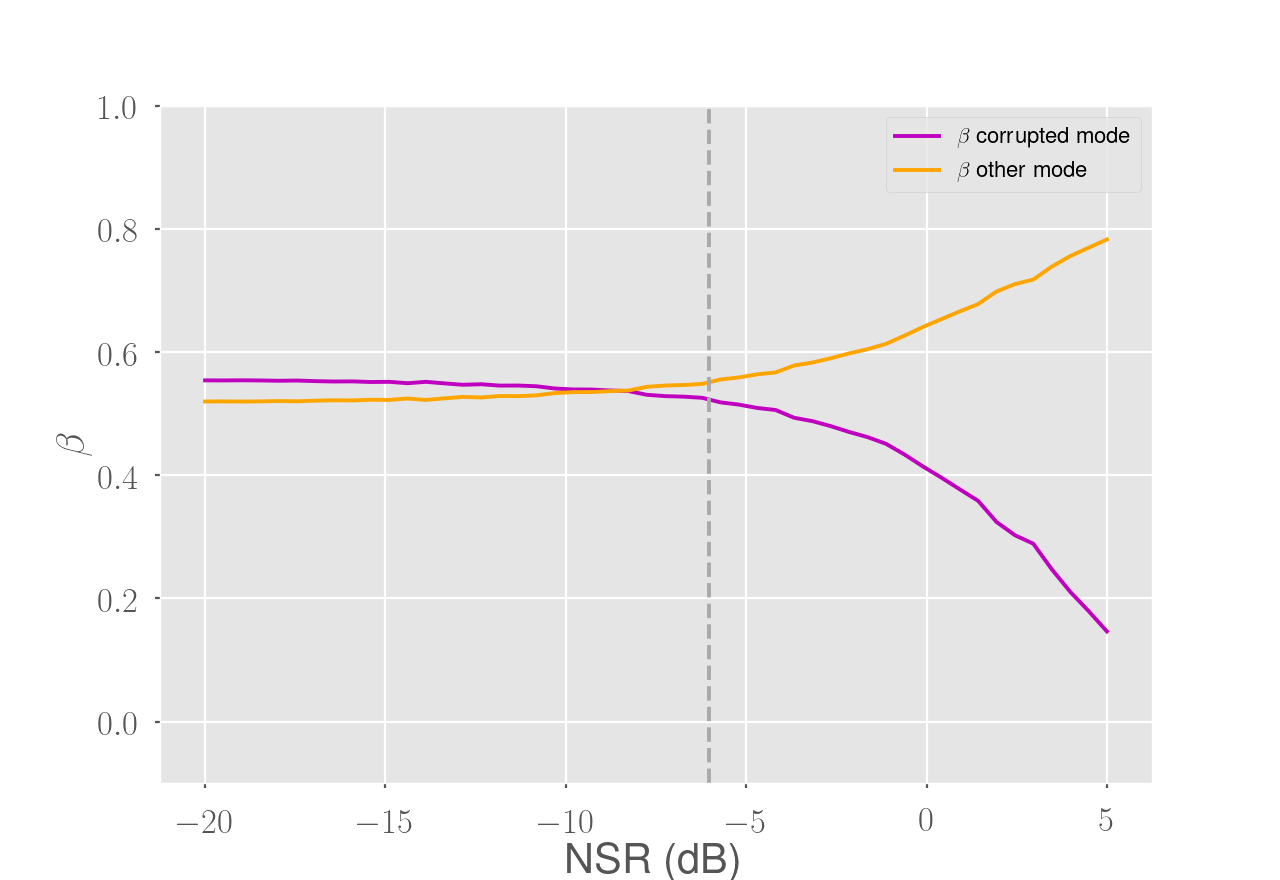
\includegraphics[width=\linewidth]{figures/new/normal-ip-noisy-beta}
  \caption{attention score, noisy IP-mode}
   \label{fig:exp-att-shift-6-c} 
\end{subfigure}%
\begin{subfigure}{.5\textwidth}
  \centering
  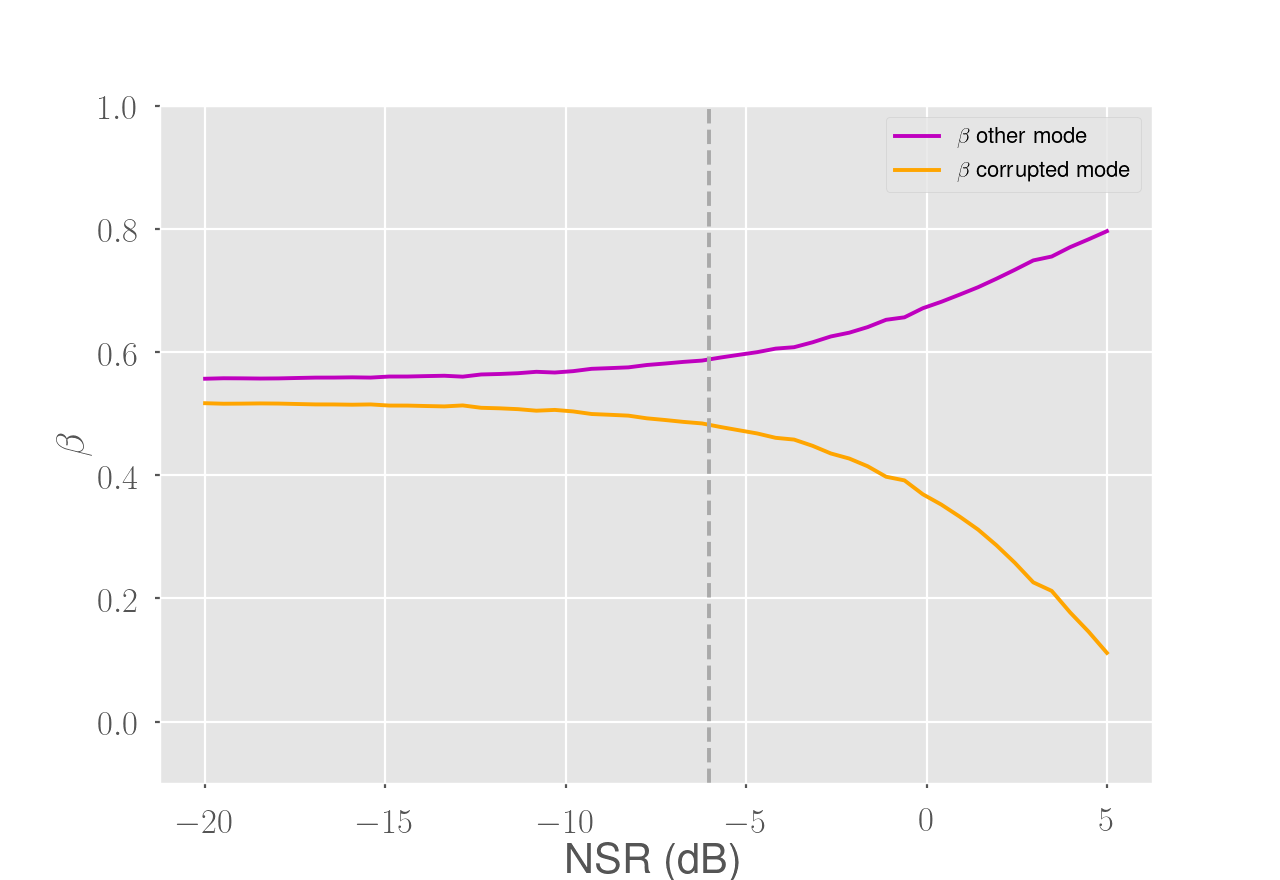
\includegraphics[width=\linewidth]{figures/new/normal-dm-noisy-beta}
  \caption{attention score, noisy DM-mode}
   \label{fig:exp-att-shift-6-d} 
\end{subfigure}
\caption[Robustness generalisation]{Robustness generalisation of \texttt{model-with} ($\rho=10^{-4},\,\lambda_e=10^{-3},\,\lambda_c=10^{-2}$). The learned capacity is 0.19.}
\label{fig:exp-att-shift-6}
\end{figure}

\subsection*{Influence of capacity regularization}
\textit{TODO: rewrite with new findings.}
\begin{figure}[!h]
\centering
\begin{subfigure}{.5\textwidth}
  \centering
  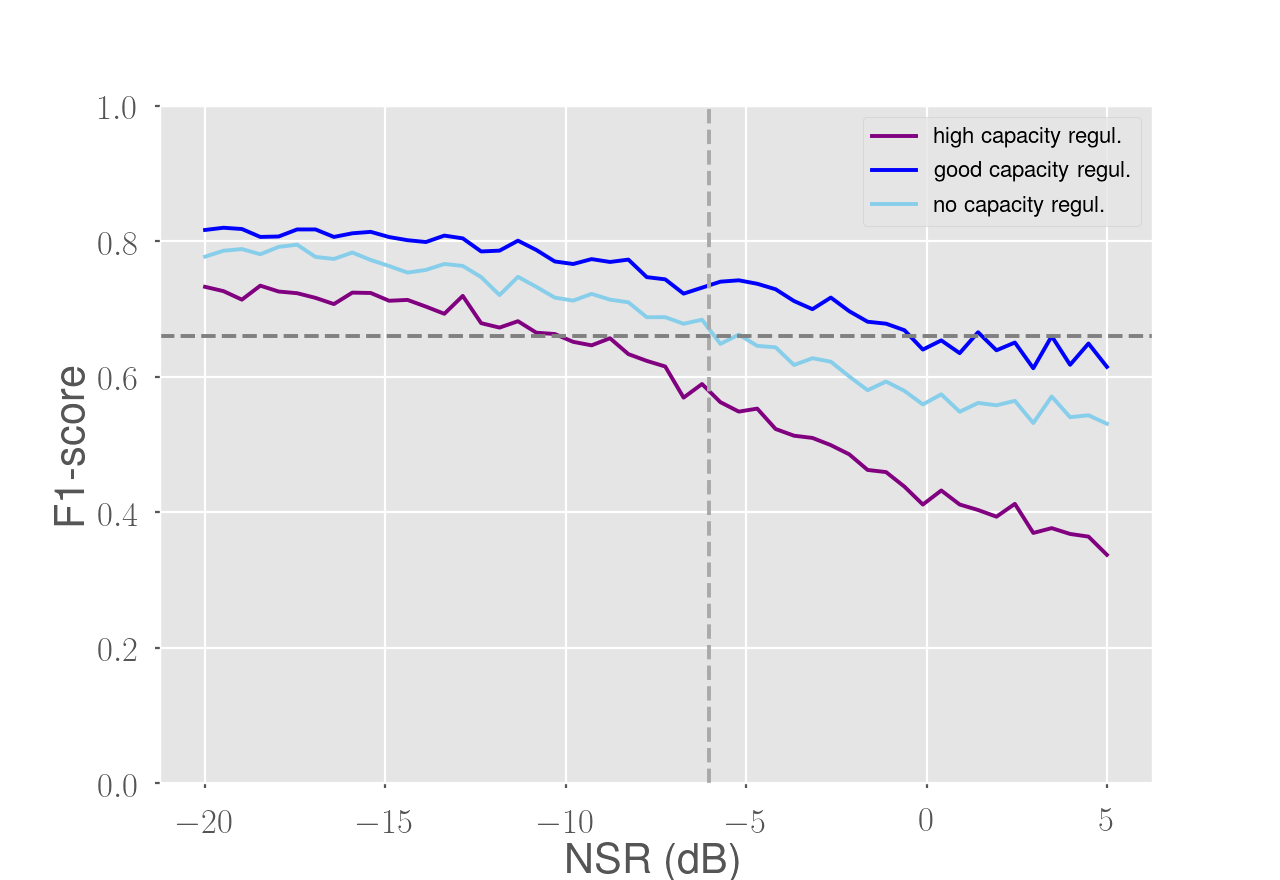
\includegraphics[width=\linewidth]{figures/new/capacity-ip-noisy}
  \caption{F1-score, noisy IP-mode}
  \label{fig:exp-att-shift-7-a}
\end{subfigure}%
\begin{subfigure}{.5\textwidth}
  \centering
  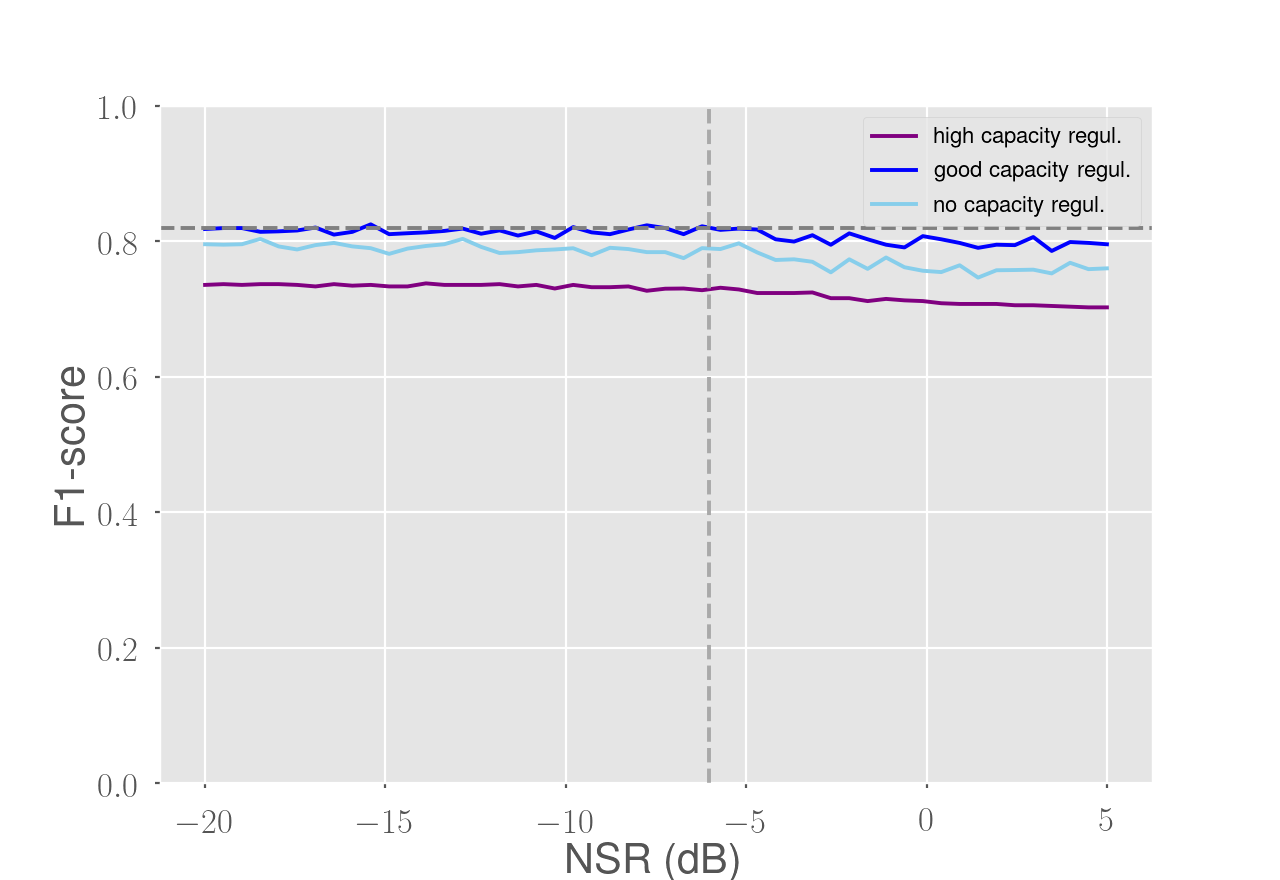
\includegraphics[width=\linewidth]{figures/new/capacity-dm-noisy}
  \caption{F1-score, noisy DM-mode}
  \label{fig:exp-att-shift-7-b}
\end{subfigure}
\caption[Influence of capacity regularization]{Influence of capacity regularizer on F1-score of \texttt{model-with} ($\rho=10^{-4},\,\lambda_e=10^{-3}$).}
\label{fig:exp-att-shift-7}
\end{figure}

\subsection*{Influence of energy regularization}
\textit{TODO: rewrite with new findings.}

\begin{figure}[!h]
\centering
\begin{subfigure}{.5\textwidth}
  \centering
  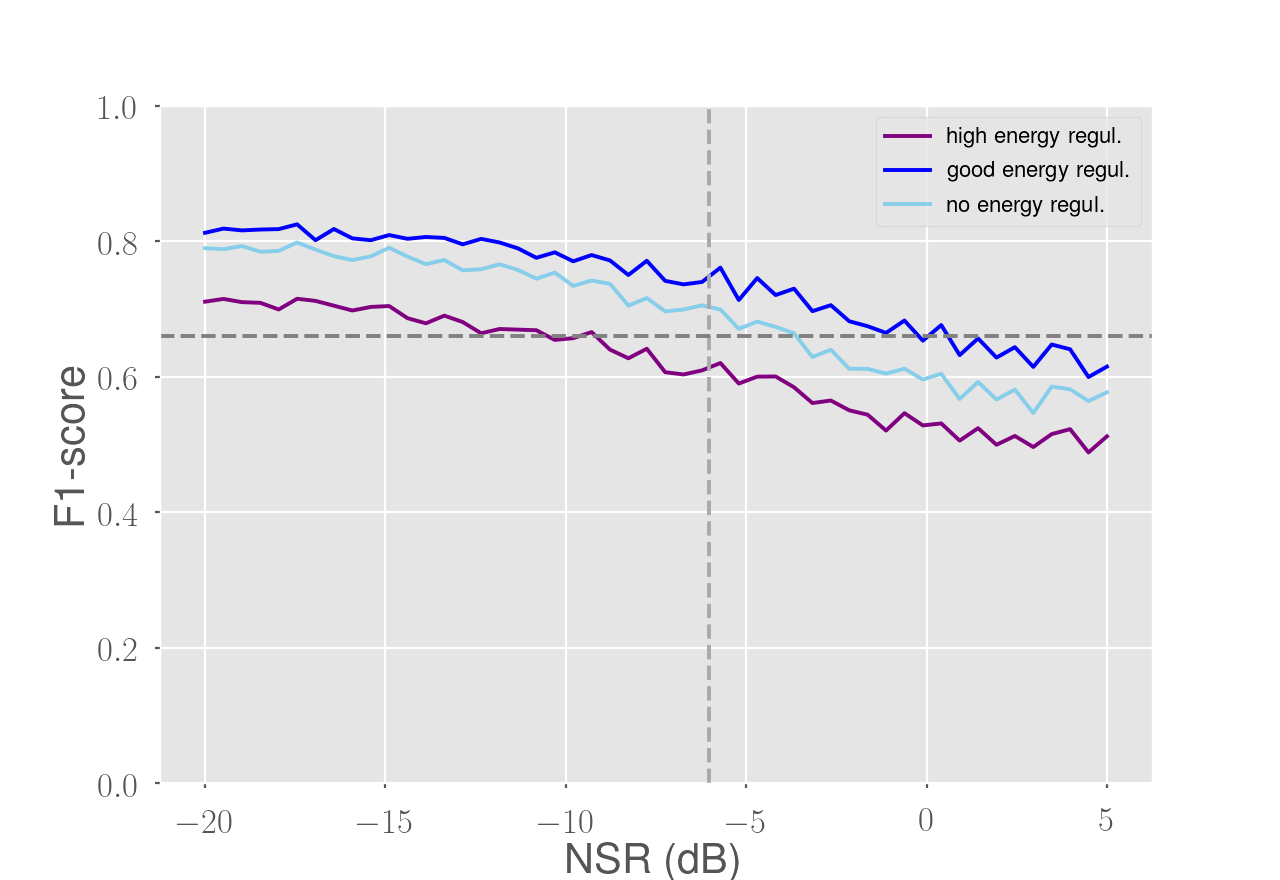
\includegraphics[width=\linewidth]{figures/new/energy-ip-noisy}
  \caption{F1-score, noisy IP-mode}
\end{subfigure}%
\begin{subfigure}{.5\textwidth}
  \centering
  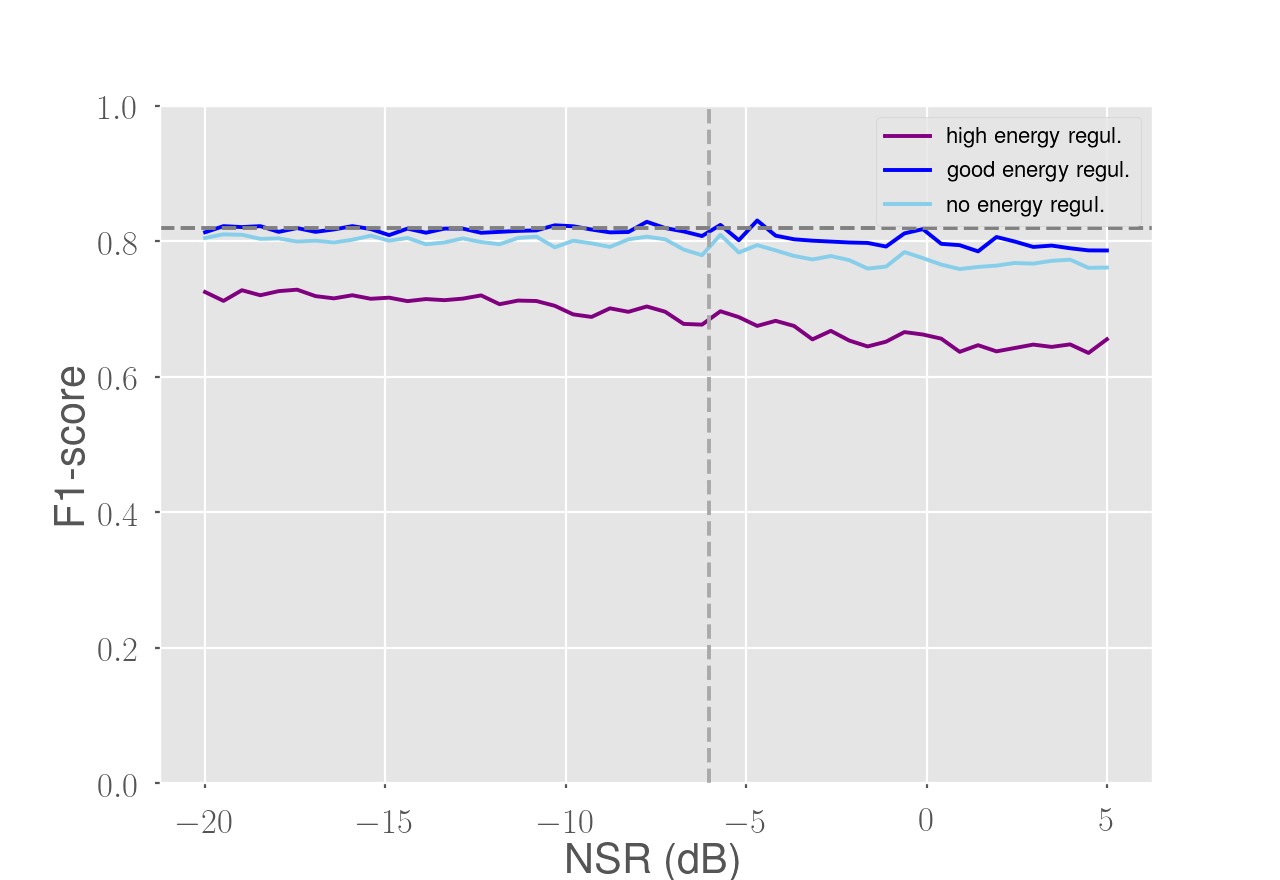
\includegraphics[width=\linewidth]{figures/new/energy-dm-noisy}
  \caption{F1-score, noisy DM-mode}
\end{subfigure}
\caption[Influence of energy regularization]{Influence of energy regularizer on F1-score of \texttt{model-with} ($\rho=10^{-4},\,\lambda_c=10^{-2}$).}
\label{fig:exp-att-shift-8}
\end{figure}


\section{Results discussion}
In the preceding sections, a set of numerical experiments was carried out in order to evaluate the performance of a novel module (EMMA) specifically designed to tackle the problem of failing modes in multi-modal deep learning approaches.

The experiments made use of a real dataset drawn from the field of astrophysics, and each sample comprised two distinct modes. Encouraging results were observed and reported, as MMN models fitted with the attention module displayed improved predictive performance, robustness, interpretability and consistently outperformed i) a traditional stand-alone MMN ii) a stand-alone MMN trained via a standard data augmentation technique. The influence of custom regularizers and related hyperparameters was also investigated.

The main objective of this work was to develop ideas and a new framework to tackle the problem of failing modes in multi-modal data. In this chapter, we believe to have verified to validity of certain of the ideas outlined in Chapter \ref{chapter-emma}. Indeed, it was shown that EMMA improves the robustness against failing modes by masking them out, these inputs were then fed to an MMN who was then able to make more stable predictions. In addition, the impact of some of the hyperparameters were discussed. However, all these results must be interpreted with caution as no general rigorous analysis was performed on a real-case dataset. Furthermore, interpreting the effect of the hyperparameters is difficult since their influence are not isolated. A limitation of the experiments that can be noticed is that the dataset only contains two modes. As a result, no complex dependencies between the modes had to be learn, minimizing the impact of the shared energies which could thus not be studied. 


\begin{figure}[!h]
\centering
\begin{subfigure}{.5\textwidth}
  \centering
  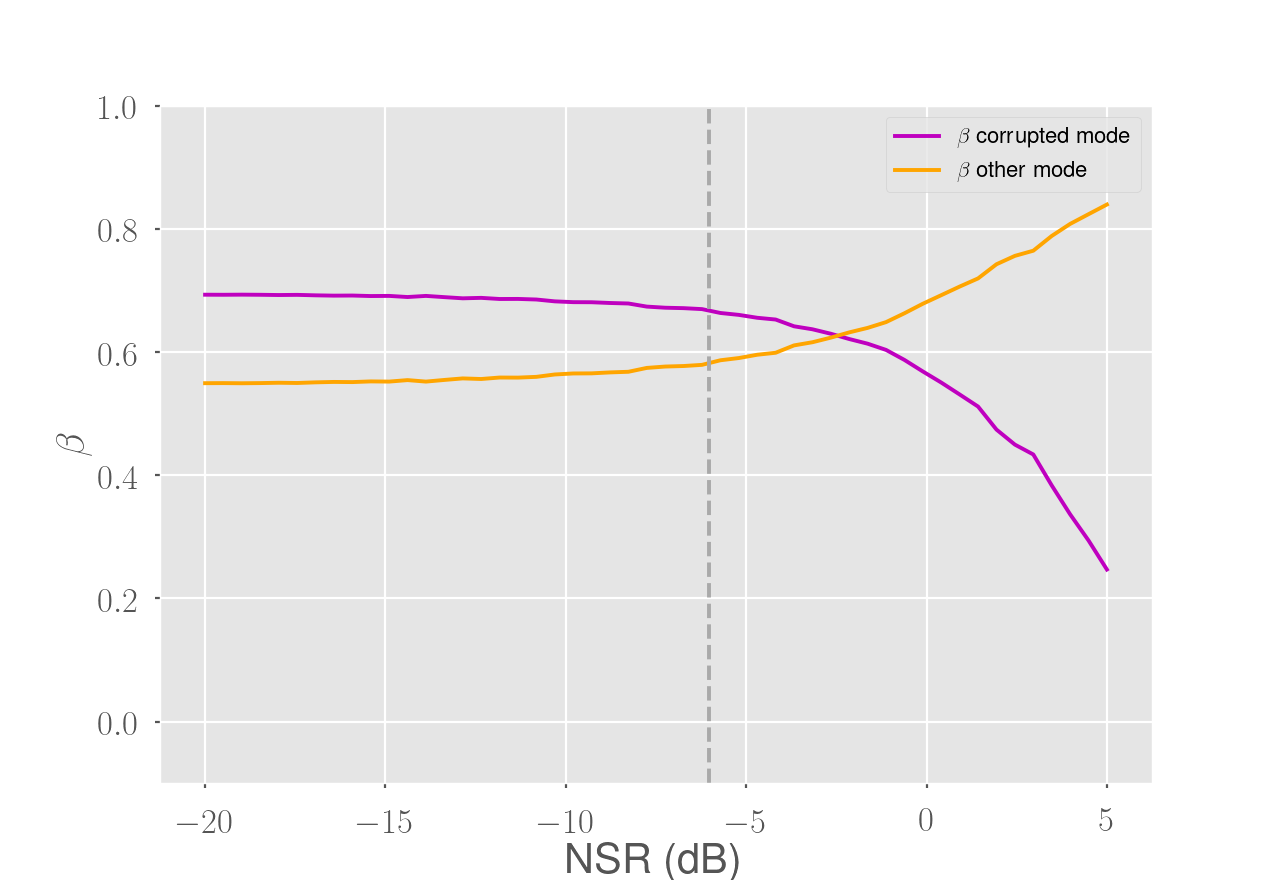
\includegraphics[width=\linewidth]{figures/new/no-capacity-ip-noisy-beta}
  \caption{F1-score, noisy IP-mode}
  \label{fig:exp-9-a}
\end{subfigure}%
\begin{subfigure}{.5\textwidth}
  \centering
  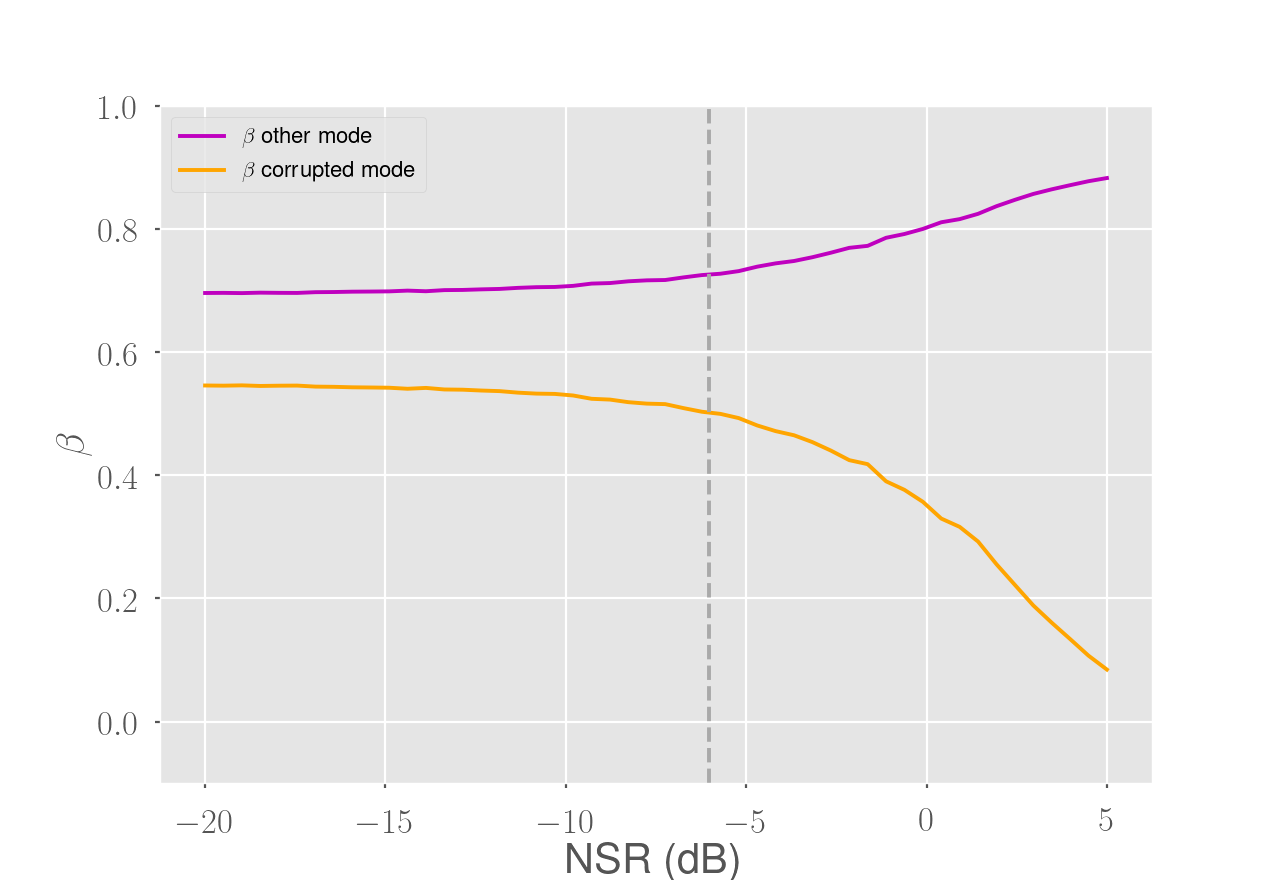
\includegraphics[width=\linewidth]{figures/new/no-capacity-dm-noisy-beta}
  \caption{F1-score, noisy DM-mode}
 \label{fig:exp-9-b} 
\end{subfigure}
\begin{subfigure}{.5\textwidth}
  \centering
  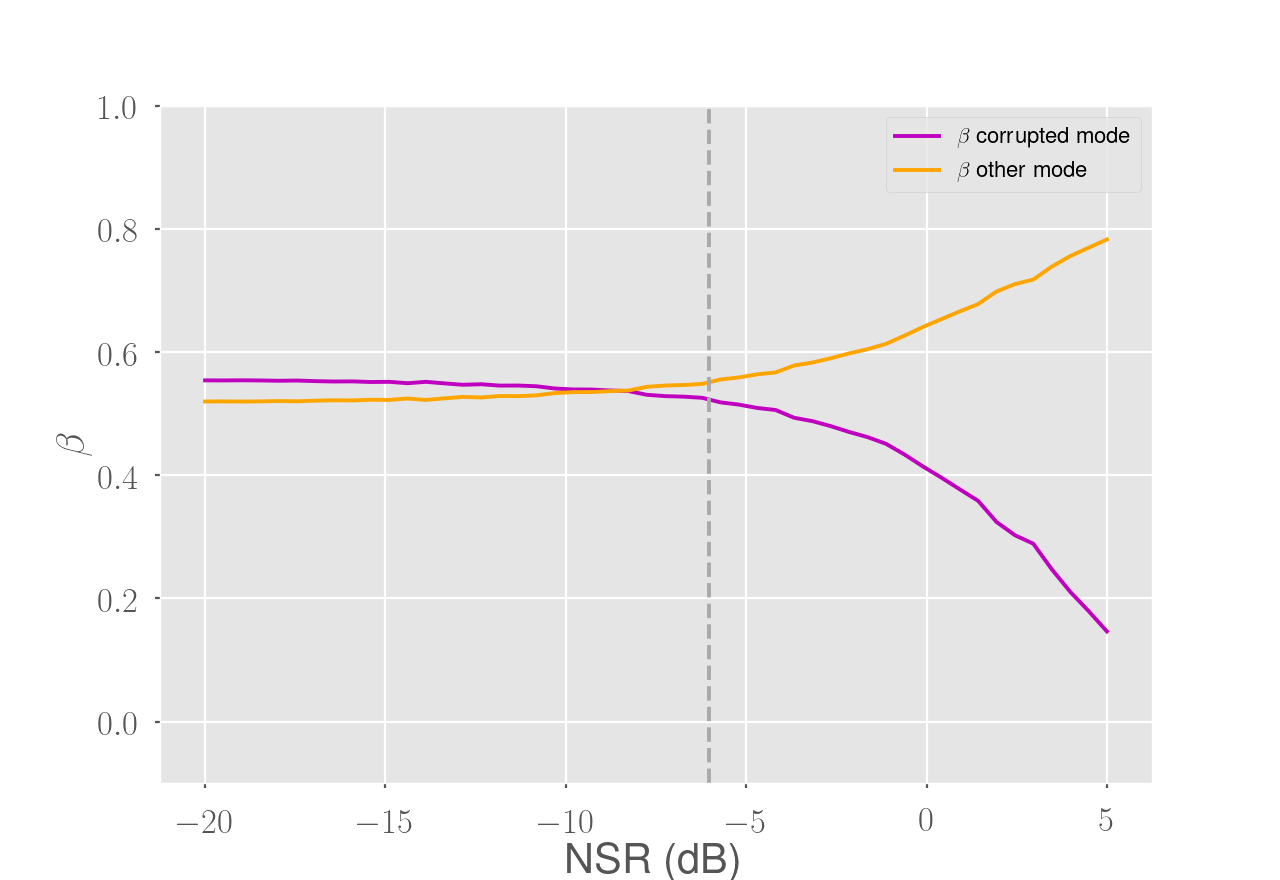
\includegraphics[width=\linewidth]{figures/new/normal-ip-noisy-beta}
  \caption{attention score, noisy IP-mode}
   \label{fig:exp-9-c} 
\end{subfigure}%
\begin{subfigure}{.5\textwidth}
  \centering
  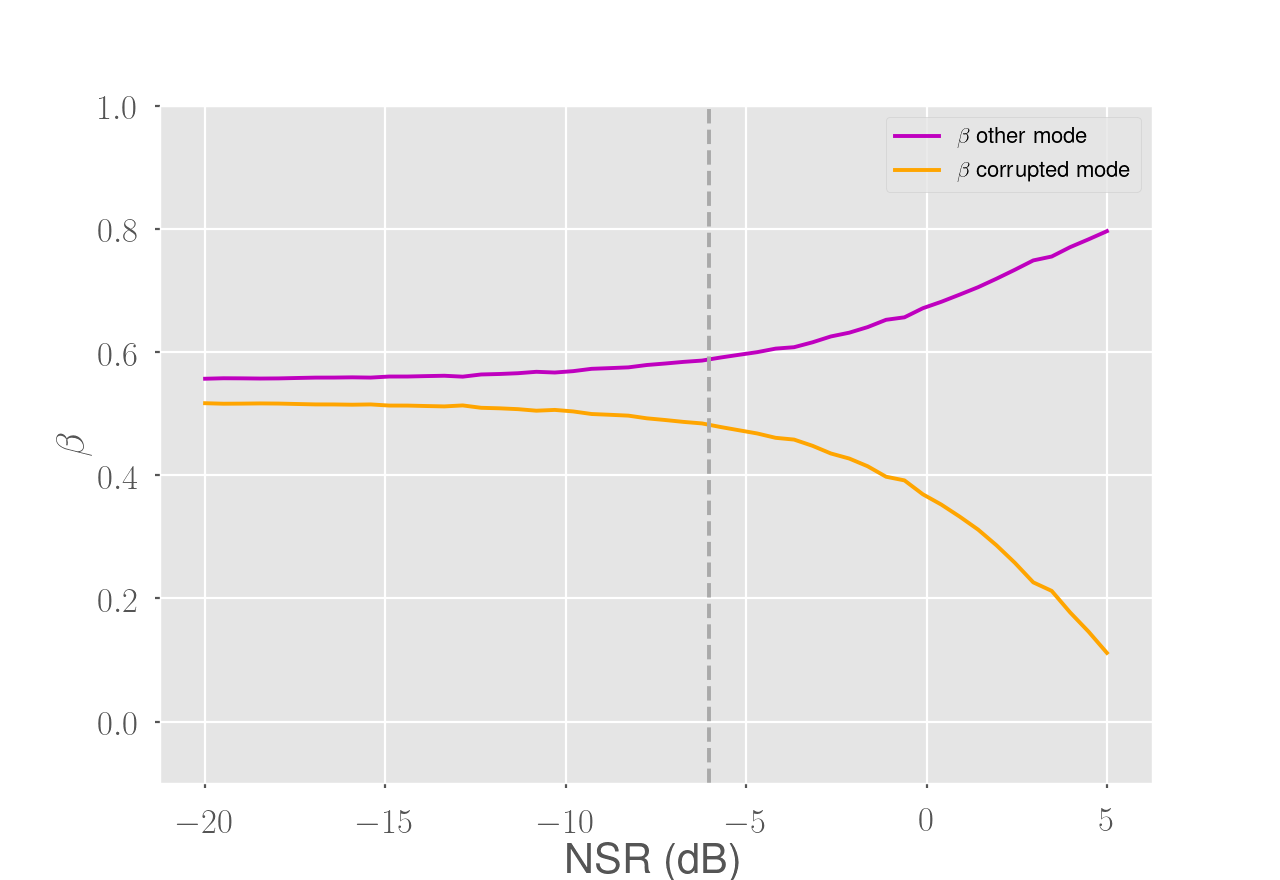
\includegraphics[width=\linewidth]{figures/new/normal-dm-noisy-beta}
  \caption{attention score, noisy DM-mode}
   \label{fig:exp-9-d} 
\end{subfigure}
\begin{subfigure}{.5\textwidth}
  \centering
  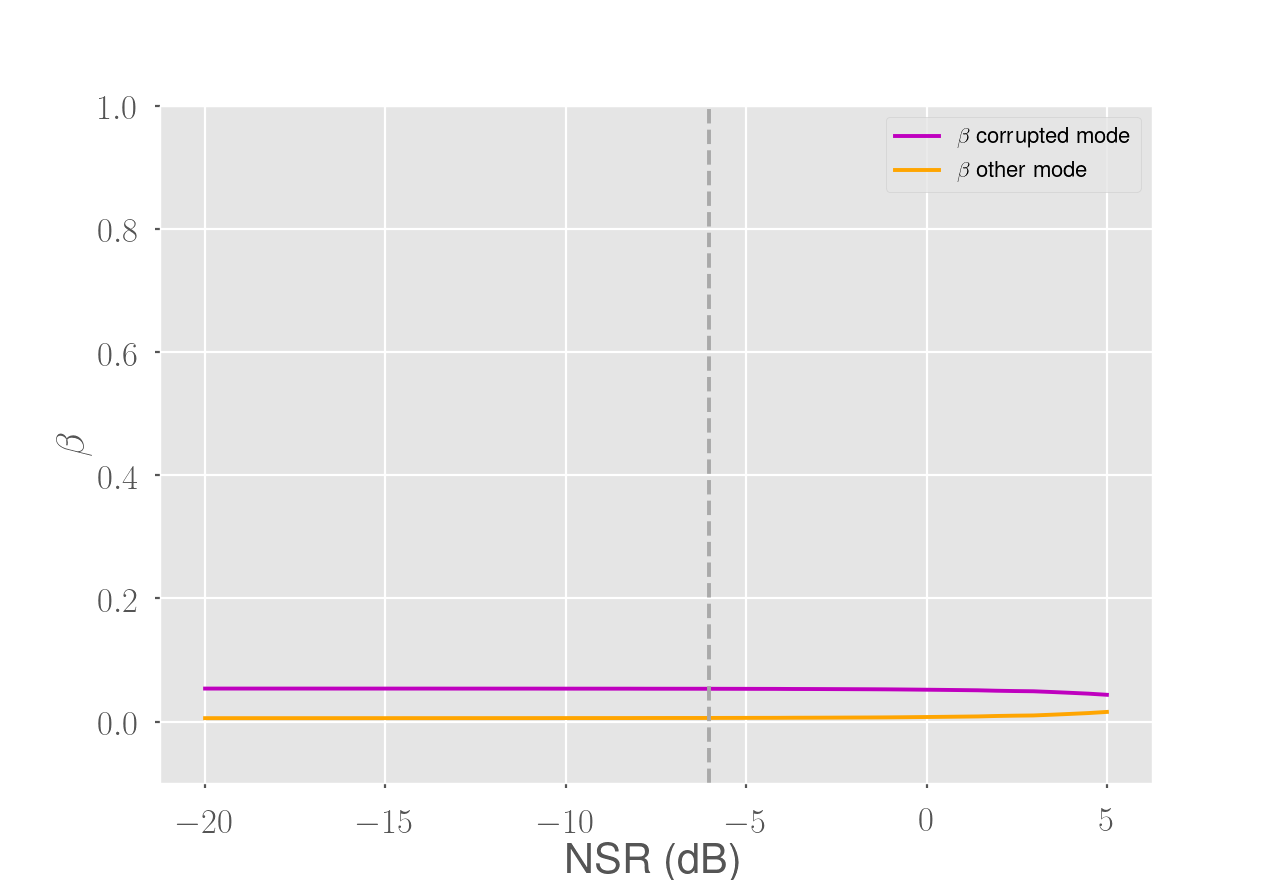
\includegraphics[width=\linewidth]{figures/new/high-capacity-ip-noisy-beta}
  \caption{attention score, noisy IP-mode}
   \label{fig:exp-9-e} 
\end{subfigure}%
\begin{subfigure}{.5\textwidth}
  \centering
  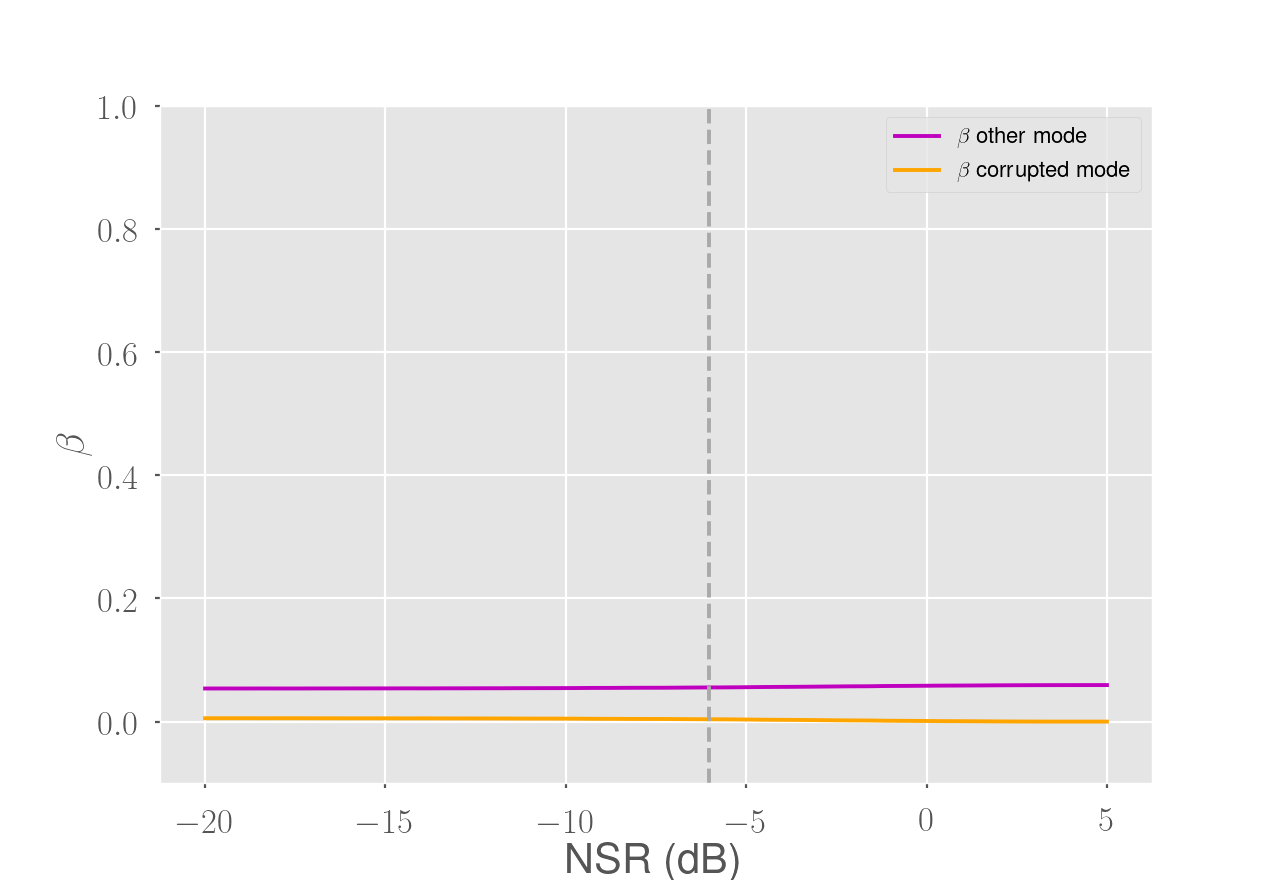
\includegraphics[width=\linewidth]{figures/new/high-capacity-dm-noisy-beta}
  \caption{attention score, noisy DM-mode}
   \label{fig:exp-9-f} 
\end{subfigure}
\caption[Robustness generalisation]{Influence of capacity regularizer on attention scores of \texttt{model-with} ($\rho=10^{-4},\,\lambda_e=10^{-3}$).}
\label{fig:exp-9}
\end{figure}

\begin{figure}[!h]
\centering
\begin{subfigure}{.5\textwidth}
  \centering
  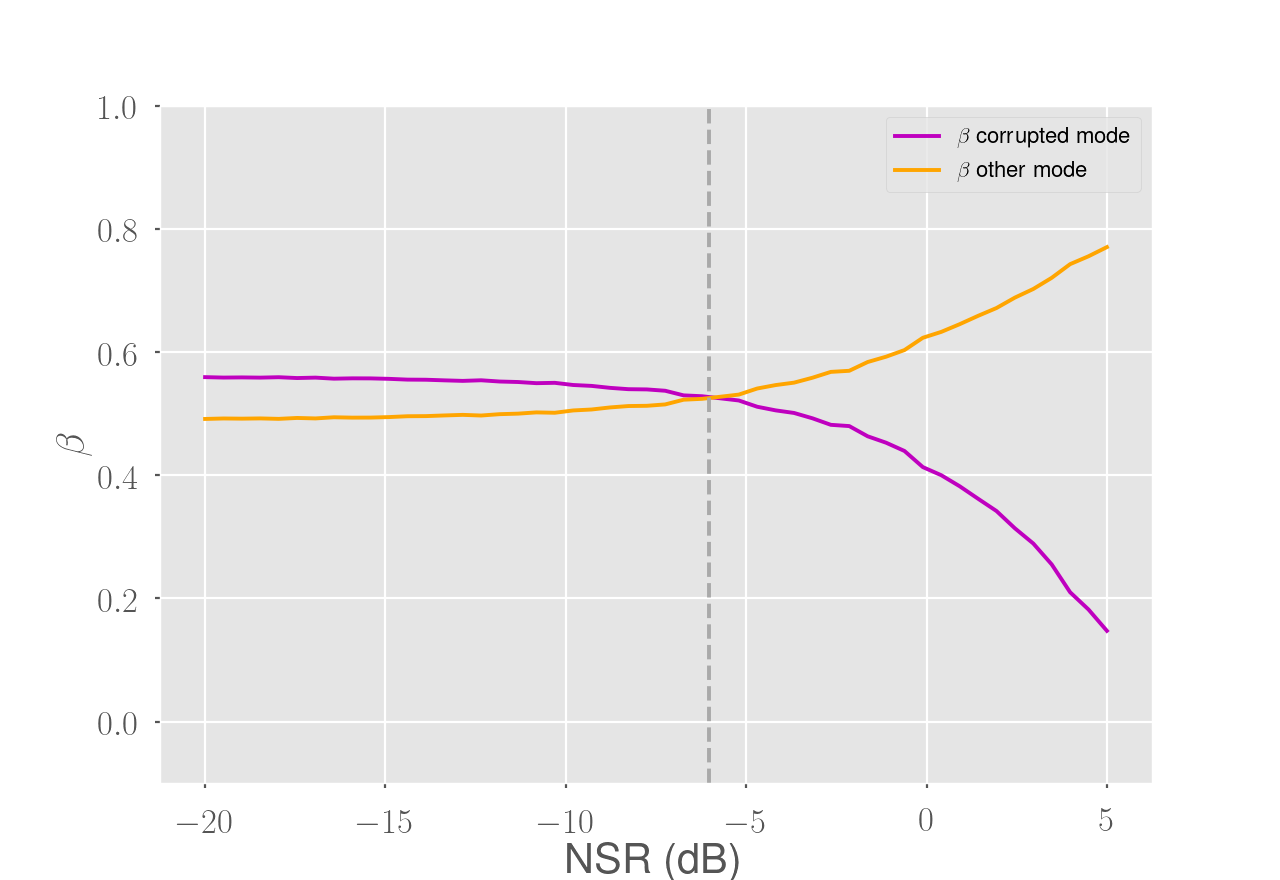
\includegraphics[width=\linewidth]{figures/new/no-energy-ip-noisy-beta}
  \caption{F1-score, noisy IP-mode}
  \label{fig:exp-10-a}
\end{subfigure}%
\begin{subfigure}{.5\textwidth}
  \centering
  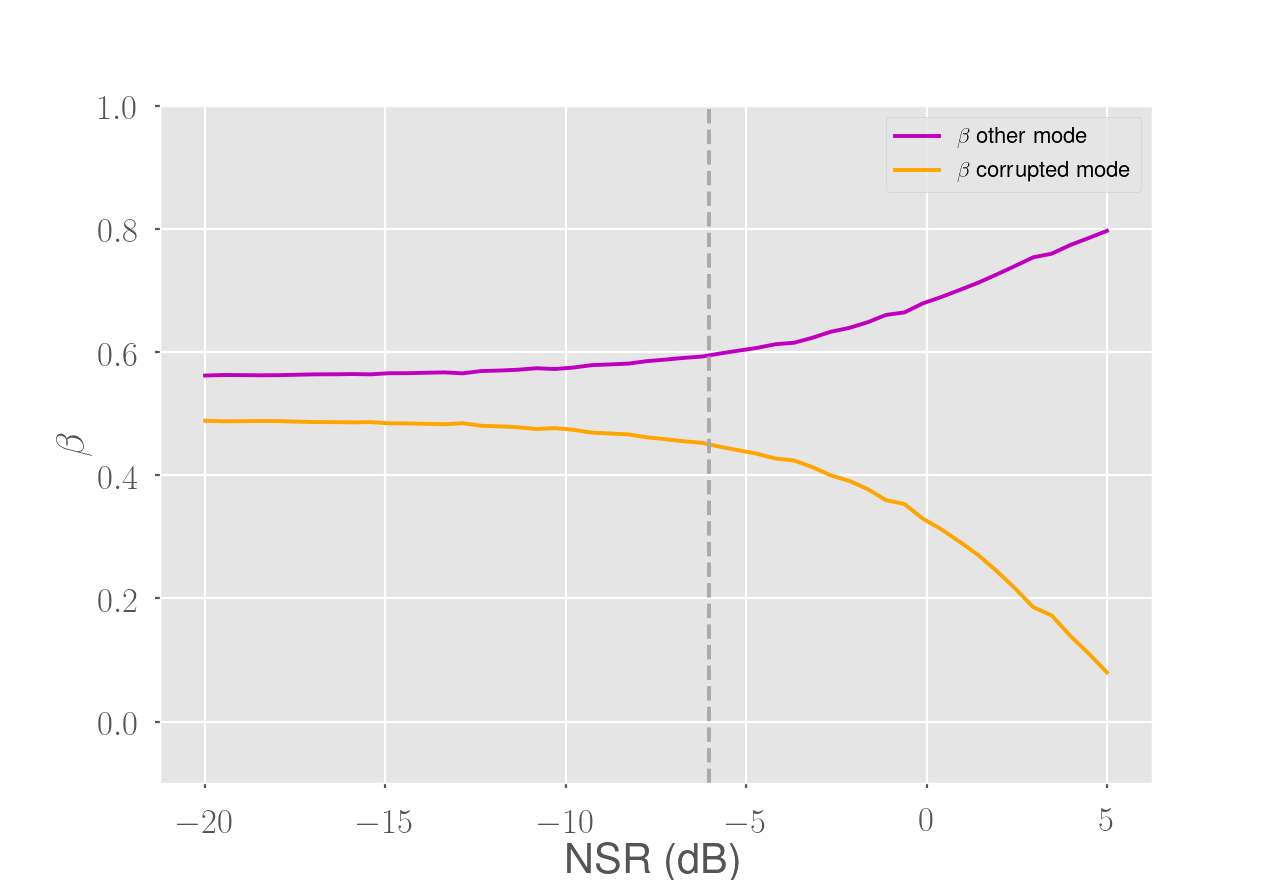
\includegraphics[width=\linewidth]{figures/new/no-energy-dm-noisy-beta}
  \caption{F1-score, noisy DM-mode}
 \label{fig:exp-10-b} 
\end{subfigure}
\begin{subfigure}{.5\textwidth}
  \centering
  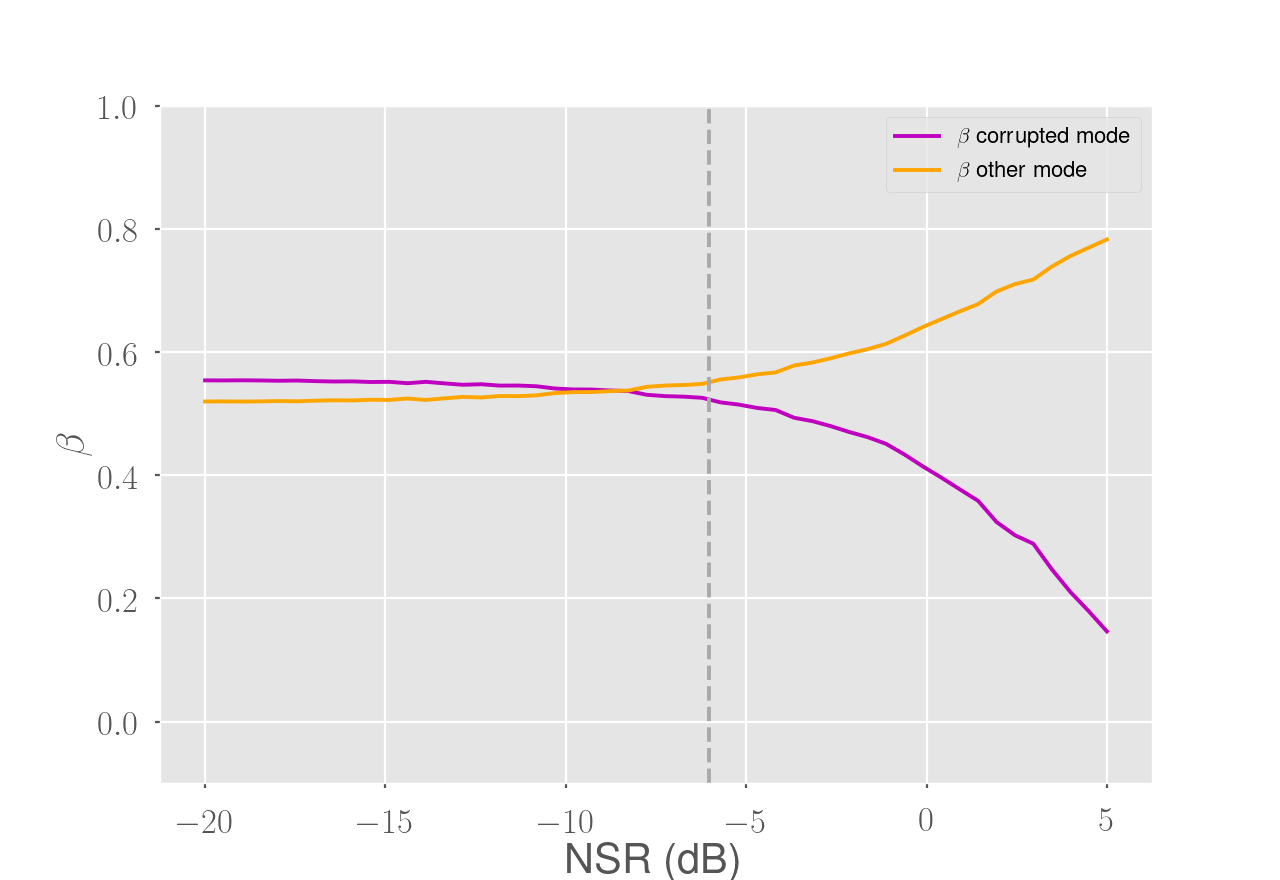
\includegraphics[width=\linewidth]{figures/new/normal-ip-noisy-beta}
  \caption{attention score, noisy IP-mode}
   \label{fig:exp-10-c} 
\end{subfigure}%
\begin{subfigure}{.5\textwidth}
  \centering
  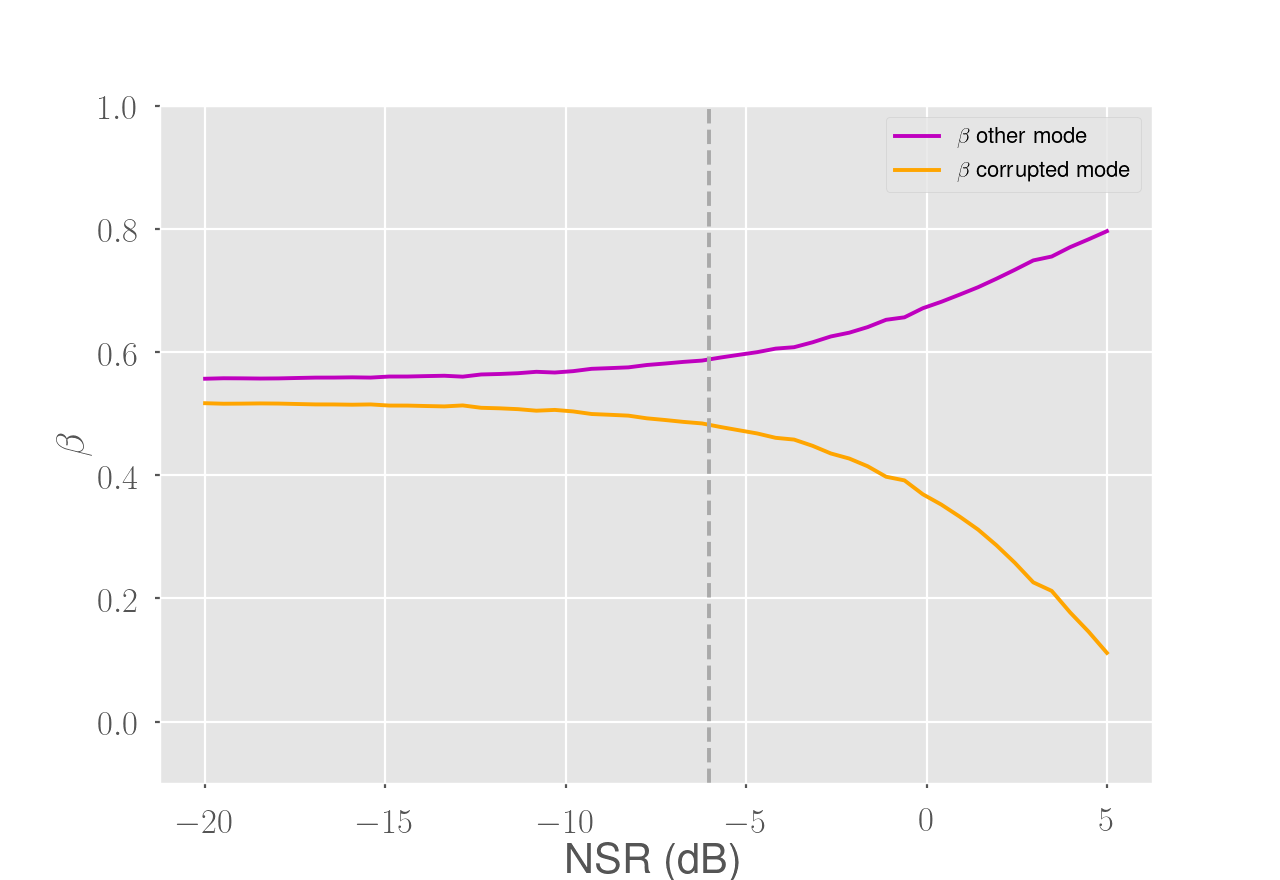
\includegraphics[width=\linewidth]{figures/new/normal-dm-noisy-beta}
  \caption{attention score, noisy DM-mode}
   \label{fig:exp-10-d} 
\end{subfigure}
\begin{subfigure}{.5\textwidth}
  \centering
  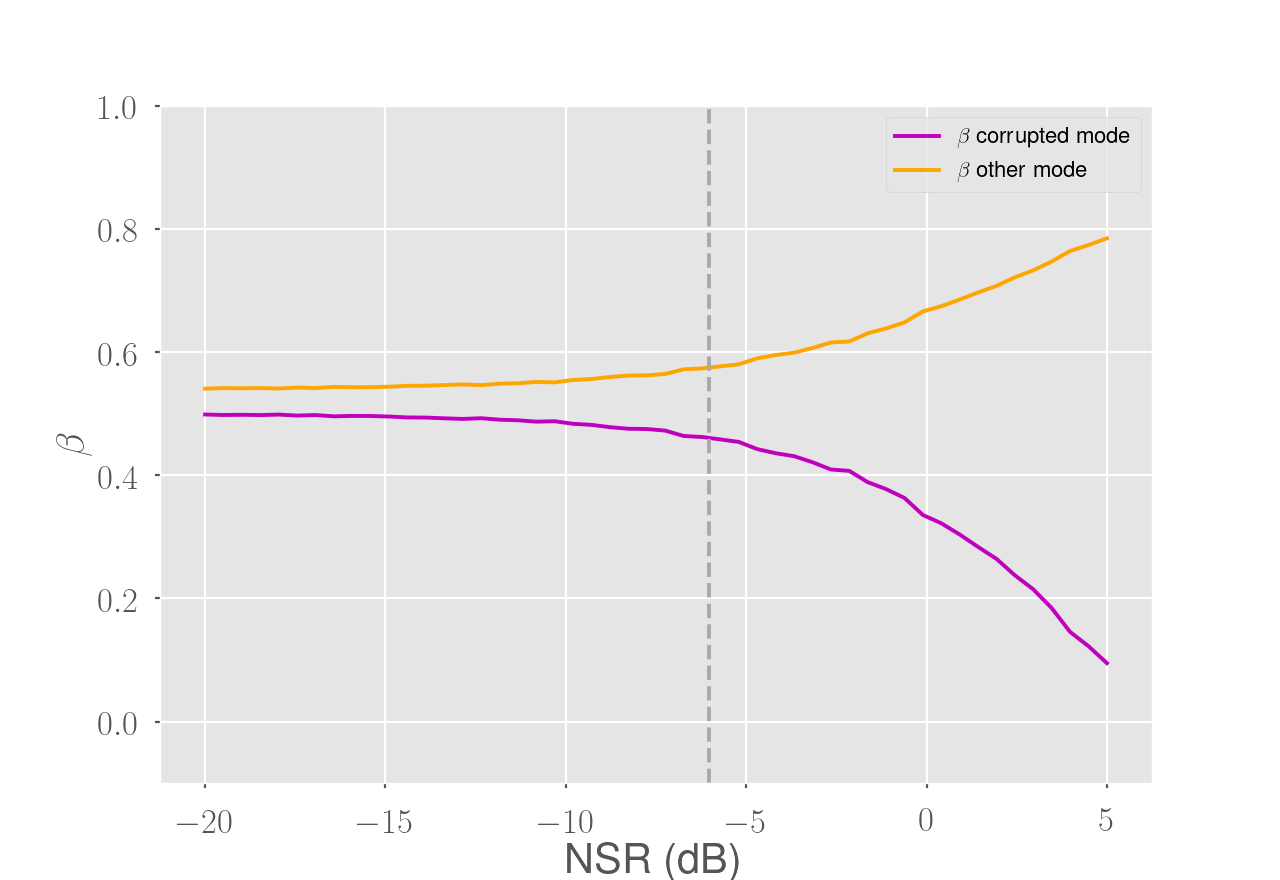
\includegraphics[width=\linewidth]{figures/new/high-energy-ip-noisy-beta}
  \caption{attention score, noisy IP-mode}
   \label{fig:exp-10-e} 
\end{subfigure}%
\begin{subfigure}{.5\textwidth}
  \centering
  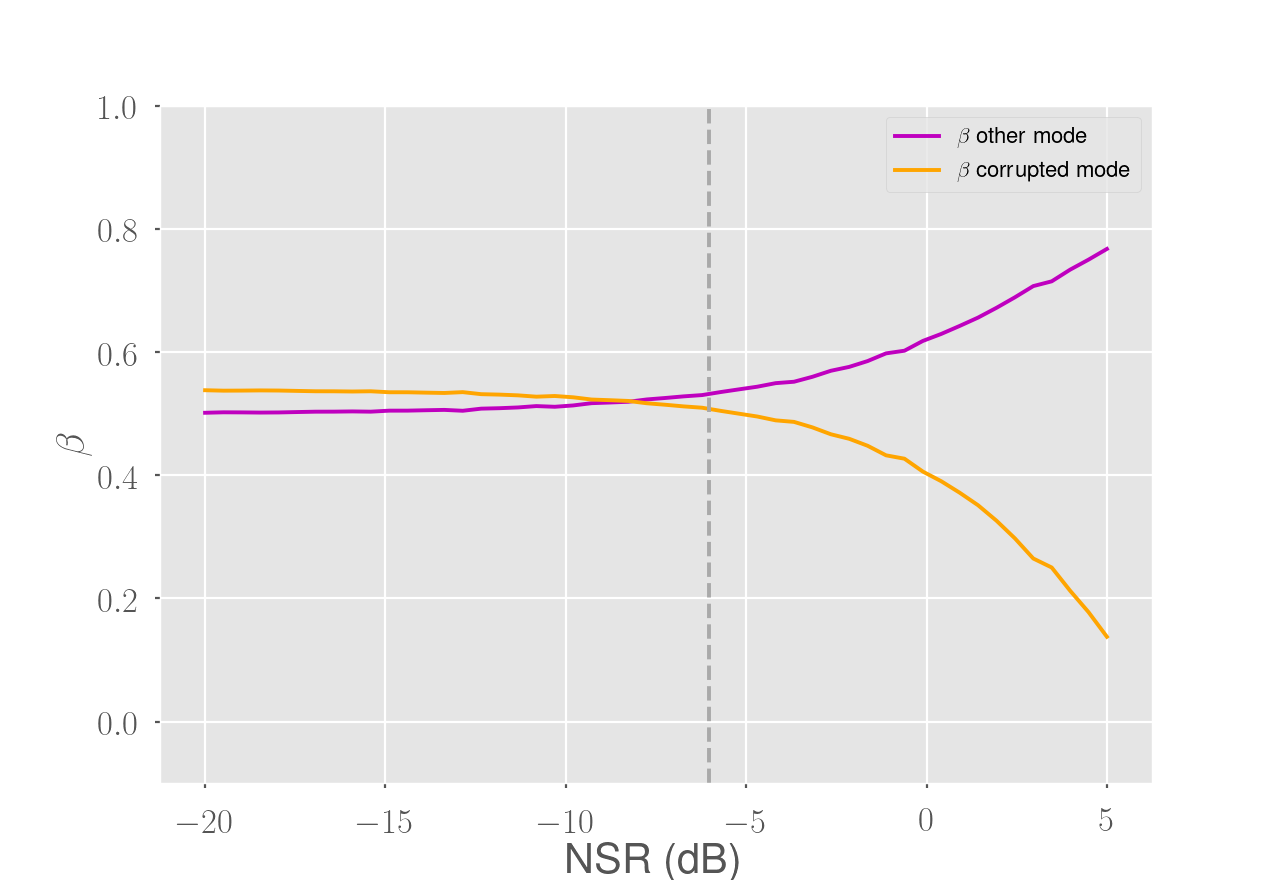
\includegraphics[width=\linewidth]{figures/new/high-energy-dm-noisy-beta}
  \caption{attention score, noisy DM-mode}
   \label{fig:exp-10-f} 
\end{subfigure}
\caption[Robustness generalisation]{Influence of energy regularizer on attention scores of \texttt{model-with} ($\rho=10^{-4},\,\lambda_c=10^{-2}$).}
\label{fig:exp-10}
\end{figure}

